\chapter{Réalisation}
\begin{spacing}{1.2}
\minitoc
\thispagestyle{MyStyle}
% \setstretch{1.2} 
\end{spacing}
\newpage
\justifying

\sloppy \setstretch{1.3} 
\section{Introduction}
\section{Prétraitement des données}

Le prétraitement des données est essentiel pour garantir la qualité des informations avant l'analyse. Il permet de nettoyer et transformer les données brutes pour qu'elles soient prêtes pour la modélisation.

\subsection{Préparation et nettoyage des données}

Chez Ooredoo, le traitement des données s'effectue via \textbf{SAS Viya}, un outil de data mining. J'ai utilisé cet outil pour accéder aux bibliothèques de données et manipuler les tables. Les enquêtes sur la satisfaction client, menées mensuellement, offrent un aperçu des raisons de satisfaction ou d'insatisfaction des services.

\textbf{Collecte des données:}
Les clients reçoivent quotidiennement un SMS les invitant à évaluer leur satisfaction sur des aspects tels que la recharge ou le réseau, avec une note globale (OSAT) de 1 à 5 :
\begin{itemize}
    \item 1: \textbf{Insatisfaction totale},
    \item 2: \textbf{Insatisfaction partielle},
    \item 3: \textbf{Neutralité},
    \item 4: \textbf{Satisfaction},
    \item 5: \textbf{Très grande satisfaction}.
\end{itemize}

Les réponses sont collectées dans des fichiers Excel, fusionnés en une table mensuelle pour analyse dans SAS.

\noindent \textbf{\(\checkmark\)} \textbf{Table mensuelle:}

La table \textbf{Resp\_Network\_Fev} contient les réponses des clients et leur score de satisfaction \textbf{OSAT}, utilisé comme \textbf{variable cible} dans notre analyse. Lors de l'importation des fichiers Excel journaliers en SAS pour les fusionner, des erreurs ont rendu la table inexploitable, par exemple, des valeurs incorrectes dans la colonne \textbf{OSAT}. On a donc développé un code pour automatiser la correction des erreurs et produire une table mensuelle propre et exploitable.


\noindent \textbf{\(\checkmark\)} \textbf{Table Monthly Aggregation:} Après avoir préparé la table \textbf{Resp\_Network\_Fev}, on a ensuite travaillé avec une autre table pour l'analyse, nommée \textbf{monthly\_aggregation}. Cette table contient des informations sur le comportement des clients au cours des trois mois précédents, notamment leur utilisation du réseau, le nombre de SMS envoyés, les montants des recharges, et d'autres indicateurs clés. 

Contrairement à la table \textbf{Resp\_Network\_Fev}, qui se concentre sur les réponses aux enquêtes, \textbf{monthly\_aggregation} regroupe des informations comportementales riches que nous utilisons comme \textbf{caractéristiques} dans notre modèle prédictif.


\noindent \textbf{\checkmark Agrégation des données:} Chaque client (identifié par \textbf{subscriber\_id}) a plusieurs enregistrements dans la table \textbf{monthly\_aggregation}, un pour chaque mois (identifié par \textbf{period\_id}). Pour obtenir une vue d'ensemble des trois mois, on a agrégé ces enregistrements en une seule ligne par client en faisant la moyenne sur les 3 mois.


Certaines variables, bien qu'utiles en théorie, posent des problèmes de crédibilité dans les données disponibles.
\noindent \textbf{\checkmark Exclusion des variables non pertinentes:}

Dans notre analyse, on a choisi de nous concentrer uniquement sur les clients prépayés en raison de leur comportement plus homogène, lié directement aux recharges. Les clients postpayés ont des comportements influencés par des offres et promotions complexes, rendant leur analyse plus difficile.

on a également exclu certaines variables qui posaient des problèmes de fiabilité ou de pertinence, telles que:
\begin{itemize}
    \item \textbf{age}, \textbf{gender}, \textbf{app\_user}, \textbf{cell\_name}, et \textbf{nom\_gouv}: Ces variables contenaient des informations souvent incomplètes ou incorrectes.
    \item \textbf{offer\_name}, \textbf{offer\_type\_name}, et \textbf{last\_offer\_id}: Variables spécifiques aux clients postpaid, non pertinentes pour notre analyse.
\end{itemize}

\noindent \textbf{\checkmark Traitement des variables:}
\begin{itemize}
    \item \textbf{Variables catégorielles:} Pour traiter les variables catégorielles, on a appliqué des transformations cohérentes. Par exemple, la variable \textbf{device\_type} a été transformée en valeurs numériques distinctes pour représenter les différents types d'appareils. Cela permet d'inclure ces variables dans les modèles prédictifs sans créer de biais.

    \begin{figure}[H]
        \centering
        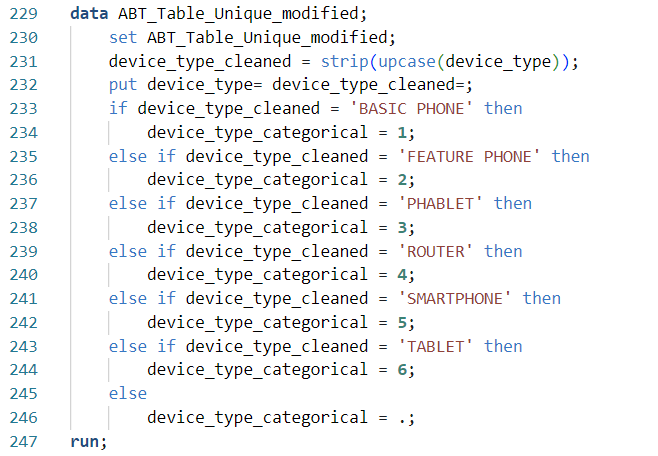
\includegraphics[width=0.5\textwidth]{capture_sas_3.png}
        \caption{Exemple de transformation des variables catégorielles}
        \label{fig:categorical_example}
    \end{figure}

    \item \textbf{Variables quantitatives:} En ce qui concerne les variables quantitatives, telles que les minutes d'appel (\textbf{mou}) ou les SMS envoyés (\textbf{number\_of\_sms}), on a procédé à une agrégation des sous-catégories pour obtenir des variables globales. Par exemple, la variable \textbf{mou\_m1} regroupe les minutes d'appels \textbf{onnet}, \textbf{offnet}, et \textbf{internationales}. Cela permet de simplifier l'analyse tout en conservant la pertinence des données.

    \begin{figure}[H]
        \centering
        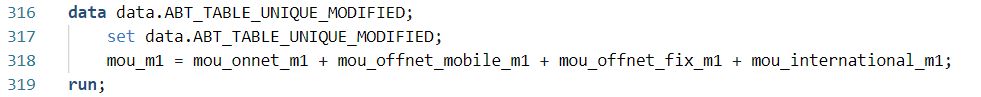
\includegraphics[width=0.7\textwidth]{capture_sas_4.png}
        \caption{Exemple d'agrégation des variables quantitatives}
        \label{fig:quantitative_example}
    \end{figure}

    \item \textbf{Variable cible binaire:} On a également créé une nouvelle variable binaire, \textbf{osat\_binary}, qui représente la satisfaction des clients de manière simplifiée. Les valeurs 1 et 2 de la variable \textbf{OSAT} sont considérées comme insatisfaction (codées par 1), tandis que les valeurs 3, 4 et 5 sont regroupées sous la catégorie satisfaction (codées par 0). Cette transformation facilite l'application de modèles de classification binaire.

\end{itemize}

Ces transformations garantissent que les données, tant qualitatives que quantitatives, sont consolidées et normalisées pour assurer une analyse cohérente et robuste.


\noindent \textbf{\checkmark Fusion des tables et agrégation:} on a fusionner les tables \textbf{Resp\_Network\_Fev} et \textbf{monthly\_aggregation} pour obtenir une table finale. La variable \textbf{OSAT} est extraite de \textbf{Resp\_Network\_Fev} et intégrée dans la table finale. Celle-ci contient les comportements clients sur plusieurs mois ainsi que leur score de satisfaction.
La table finale agrégée comprend \textbf{25 colonnes} et \textbf{985 lignes}. Elle regroupe les informations prêtes pour l'analyse. Voici les colonnes principales :

\begin{longtable}{|p{7cm}|p{9cm}|}
    \hline
    \textbf{Nom de la variable} & \textbf{Description} \\ \hline
    \textbf{msisdn} & Identifiant unique du client \\ \hline
    \textbf{OSAT} & Score de satisfaction global \\ \hline
    \textbf{subscriber\_activation\_date\_only} & Date d'activation du client \\ \hline
    \textbf{Indicator\_vas} & Utilisation des services à valeur ajoutée \\ \hline
    \textbf{monthly\_rech\_subscriber\_seg} & Montant moyen des recharges mensuelles \\ \hline
    \textbf{monthly\_arpu\_subscriber\_seg} & Revenu moyen par utilisateur \\ \hline
    \textbf{Number\_of\_reactivation} & Nombre de réactivations \\ \hline
    \textbf{Flag\_4g\_binary} & Utilisation de la 4G (binaire) \\ \hline
    \textbf{device\_type} & Type d'appareil \\ \hline
    \textbf{flag\_smartphone} & Indique un smartphone \\ \hline
    \textbf{recharge\_moyenne} & Montant moyen des recharges \\ \hline
    \textbf{Arpu\_moyenne} & Revenu moyen \\ \hline
    \textbf{data\_volume\_moyenne} & Volume moyen de données \\ \hline
    \textbf{mou\_moyenne} & Moyenne des minutes d'appels \\ \hline
    \textbf{nbre\_recharges\_moyenne} & Nombre moyen de recharges \\ \hline
    \textbf{nbre\_sms\_moyenne} & Nombre moyen de SMS \\ \hline
    \textbf{voice\_amount\_moyenne} & Montant moyen des appels vocaux \\ \hline
    \textbf{data\_amount\_moyenne} & Montant moyen des données utilisées \\ \hline
    \textbf{voice\_volume\_moyenne} & Volume moyen des appels \\ \hline
\caption{Colonnes principales de la table finale.}
\label{table:variables_final}
\end{longtable}
\textbf{\checkmark Gestion des valeurs manquantes:}
\begin{enumerate}
    \item \textbf{Imputation pour OSAT:} Certaines lignes de la table \textbf{Resp\_Network\_Fev} contenaient des valeurs manquantes dans la colonne \textbf{OSAT}. On a imputé ces valeurs en utilisant la moyenne des réponses aux questions \textbf{q3} à \textbf{q18}. Le code complet pour cette imputation est disponible dans l'annexe (voir figure \ref{imputation_code}).

    \item \textbf{Imputation pour subscriber\_activation\_date\_only:} Un total de \textbf{114 valeurs manquantes} a été détecté dans cette colonne. Pour y remédier, on a utilisé \textbf{KNNImputer} et l'imputation par la médiane via \textbf{Jupyter Notebook}. 

    Avant l'imputation, les dates ont été converties en jours depuis une date de référence (\textbf{01/01/1970}), créant une variable \textbf{activation\_days}. La colonne d'origine a ensuite été supprimée.

    \textbf{Imputation KNN:} On a appliqué \textbf{KNNImputer} avec 5 voisins pour estimer les valeurs manquantes, en se basant sur la similarité avec les autres colonnes. Pour le code complet utilisé dans cette méthode, référez-vous à la figure \ref{fig:knn_code} dans l'annexe.

    \textbf{Imputation par la médiane:} En complément, on a testé l'imputation par la médiane pour comparer avec KNN et identifier la méthode la plus fiable.

\end{enumerate}

\subsection{Normalisation des données}

La normalisation est essentielle pour rendre les variables comparables et améliorer les performances des algorithmes d'apprentissage.

\textbf{\checkmark Gestion des valeurs aberrantes:}  
On a identifié et remplacé les valeurs aberrantes des variables quantitatives (montants de recharge, volume de données, SMS, minutes d'appels) en utilisant les quartiles (\textbf{Q1}, \textbf{Q3}) et l'intervalle interquartile (\textbf{IQR}). Les valeurs en dehors de l'intervalle (\textbf{Q1 - 1.5 * IQR} à \textbf{Q3 + 1.5 * IQR}) ont été remplacées par la médiane pour éviter les biais. Le code utilisé pour cette étape est disponible dans l'annexe (voir figure \ref{fig:aberrant_values_annex}).

\textbf{\checkmark Normalisation Box-Cox:}  
Après avoir géré les valeurs aberrantes, différentes méthodes de normalisation (\textbf{min-max}, \textbf{sqrt}, \textbf{log}) ont été testées sans succès. On a donc appliqué la transformation \textbf{Box-Cox}, particulièrement efficace pour les données asymétriques. L'algorithme a optimisé la valeur de \(\lambda\) à l'aide de la courbe de log-vraisemblance. La transformation a été appliquée à la variable \textbf{Recharge\_moyenne}, créant la nouvelle variable normalisée \textbf{new\_recharge\_moyenne}. Le code détaillé est présenté dans l'annexe (voir figure \ref{fig:boxcox_transformation_annex}).

Après la transformation et la gestion des valeurs aberrantes, on a vérifié la distribution des données normalisées via les histogrammes. La normalité a aussi été testée avec Shapiro-Wilk, mais les résultats ne sont pas disponibles en raison d'un problème sur la plateforme SAS en fin de stage. Cependant, les premiers résultats montrent que la normalité n'est pas totalement vérifiée, bien que les données de cette table soient presque normales. La table a été exportée en format Excel pour l'analyse et la modélisation sur Jupyter, offrant plus de flexibilité et rapidité.

\subsection{Utilisation de plusieurs tables}

\textbf{\checkmark Application sur plusieurs jeux de données:}  
Le processus de prétraitement a été appliqué à plusieurs jeux de données pour garantir la pertinence et la continuité temporelle. On a traité les tables \textbf{Resp\_Network\_Fev}, \textbf{network\_may} et \textbf{retail\_juin}, couvrant les périodes de février à juin. Chaque table contient des colonnes similaires et a été soumise au même processus de nettoyage et de transformation.

\noindent \textbf{\checkmark Comparaison des échantillons:}  
La table \textbf{network\_may} contient 375 lignes, un échantillon relativement réduit. Pour obtenir des résultats plus représentatifs, on a également utilisé \textbf{retail\_juin}, qui compte 2554 lignes. Cela permet d'analyser les variations temporelles et d'assurer la robustesse des résultats.

\noindent \textbf{\checkmark Pourquoi trois datasets ?}  
L'utilisation de ces trois tables permet de comparer les performances des modèles sur différentes périodes, d'analyser les tendances comportementales, et d'évaluer la persistance des schémas.

\noindent \textbf{Détails sur les trois tables:}  
\begin{itemize}
    \item \textbf{Resp\_Network\_Fev}: 985 lignes, 114 valeurs manquantes pour \textbf{activation\_days}.
    \item \textbf{network\_may}: 375 lignes, 44 valeurs manquantes.
    \item \textbf{retail\_juin}: 2554 lignes, 281 valeurs manquantes.
\end{itemize}

\noindent \textbf{\checkmark Difficultés de normalisation:}  
Malgré les efforts, la normalisation des données dans \textbf{network\_may} et \textbf{retail\_juin} n'a pas réussi pour certaines variables, même avec les méthodes \textbf{min-max}, \textbf{sqrt}, \textbf{log}, et \textbf{Box-Cox}. Cela sera pris en compte lors de l'analyse des résultats.

\noindent \textbf{\checkmark Travail avec les trois tables:}  
Les trois jeux de données seront utilisés pour:
\begin{itemize}
    \item Comparer les performances des modèles,
    \item Évaluer la robustesse des résultats sur plusieurs périodes,
    \item Identifier les différences comportementales entre les clients.
\end{itemize}

Ces trois jeux de données, bien que présentant des défis de normalisation, offrent une base solide pour l'analyse et la modélisation prédictive.

\section{Analyse des données}
L'analyse des données comprend à la fois une exploration descriptive des variables et une analyse inférentielle pour extraire des conclusions significatives.

\subsection{Analyse descriptive}

L'analyse descriptive a été réalisée sur la variable \textbf{recharge}, en examinant son comportement par rapport à la variable \textbf{OSAT}, à la fois en version multiclasse et binaire.
\subsubsection{Analyse des variables quantitatives}

\subsubsection*{Analyse pour la variable Recharge}
Les statistiques descriptives pour la variable \textbf{recharge} selon les classes \textbf{OSAT} multiclasse sont présentées à travers la distribution de la variable par classe dans la figure \ref{fig:analyse_descriptive_2}.

\begin{figure}[H]
    \centering
    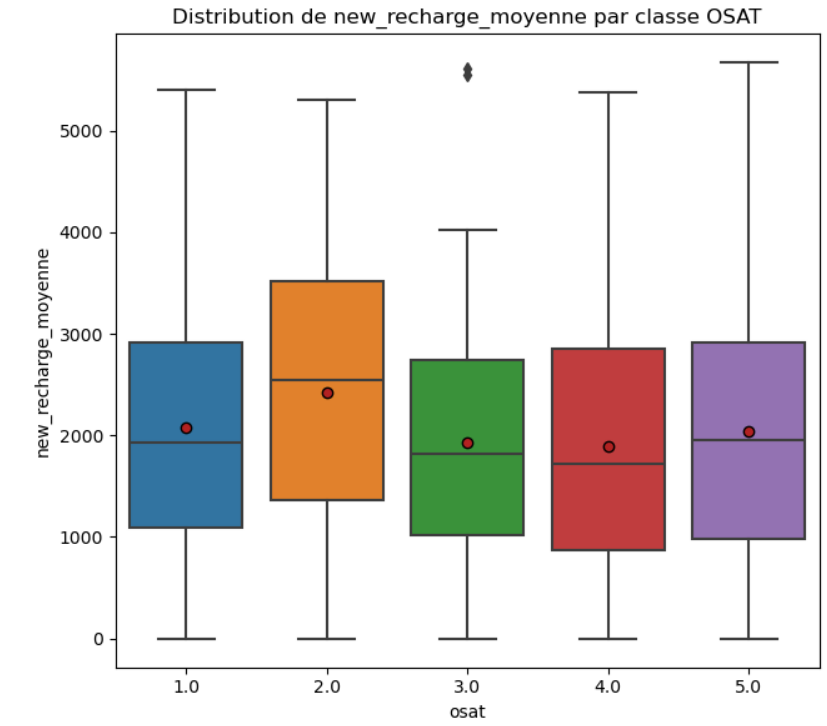
\includegraphics[width=0.7\linewidth]{analyse_descriptive_2.png}
    \caption{Distribution de la variable \textbf{recharge} par classe \textbf{OSAT} multiclasse.}
    \label{fig:analyse_descriptive_2}
\end{figure}

Les moyennes de \textbf{recharge} montrent une légère variation entre les classes \textbf{OSAT} multiclasse. Les classes 2 et 5 présentent des médianes plus élevées, tandis que la classe 1 a une médiane légèrement inférieure. Comme le montre la figure \ref{fig:analyse_descriptive_2}, la distribution de \textbf{recharge} est relativement similaire entre les classes, bien que les médianes des classes 2 et 5 soient plus élevées.

Passons maintenant à la comparaison avec \textbf{OSAT} binaire.

Les statistiques descriptives pour la variable \textbf{recharge} selon les classes \textbf{OSAT} binaire sont présentées dans le tableau ci-dessous.

\begin{table}[H]
    \centering
    \begin{tabular}{p{2cm}ccccccccc} % 9 columns
        \toprule
        Classe OSAT binaire & Nombre & Moyenne & Ecart-Type & Min & Q1 & Médiane & Q3 & Max \\
        \midrule
        0 & 334 & 2158.66 & 1323.81 & -1.33 & 1161.87 & 2041.87 & 3107.40 & 5405.60 \\
        1 & 651 & 1966.57 & 1310.51 & -1.33 & 907.64 & 1835.88 & 2881.57 & 5670.04 \\
        \bottomrule
    \end{tabular}
    \caption{Statistiques descriptives de la variable \textbf{recharge} selon la classe \textbf{OSAT} binaire.}
\end{table}

Dans la version binaire, la moyenne de \textbf{recharge} pour la classe 0 est légèrement plus élevée que celle de la classe 1, mais la variabilité est similaire entre les deux groupes, comme le montre l'écart-type.

\subsubsection*{Comparaison entre les OSAT multiclasse et OSAT binaire pour la variable recharge} 
Bien que la version multiclasse de \textbf{OSAT} offre une segmentation plus détaillée, les différences entre les classes pour la variable \textbf{recharge} ne sont pas assez marquantes pour justifier une complexité supplémentaire. Les moyennes dans la version binaire sont similaires entre les classes 0 et 1, avec une variabilité légère qui n'altère pas l'interprétation globale. Par conséquent, pour simplifier l'analyse tout en assurant une cohérence des résultats, la version binaire est privilégiée.

\subsubsection*{Analyse pour les variables quantitatives}

L'analyse des variables quantitatives selon OSAT multiclasse et OSAT binaire révèle des tendances intéressantes. Voici les points principaux :

\noindent \textbf{ARPU:} \\
\textbf{OSAT multiclasse}: L'ARPU moyen varie légèrement entre les classes (255 à 301). Les classes 2 et 5 présentent les valeurs moyennes les plus élevées, reflétant une consommation plus importante de ces groupes. \\
\textbf{OSAT binaire}: La différence entre les classes 0 et 1 est faible (278 vs 275), avec une variabilité similaire entre les deux groupes.

\vspace{0.2cm}

\noindent \textbf{Volume d'appels (voice\_volume):} \\
\textbf{OSAT multiclasse}: Les moyennes sont stables entre les classes (38 à 43), avec une légère augmentation pour les classes 4 et 5. \\
\textbf{OSAT binaire}: Différence marginale entre les classes 0 et 1 (41,27 vs 42,28), avec une distribution homogène.

\vspace{0.2cm}

\noindent \textbf{Nombre d'appels (voice\_amount):} \\
\textbf{OSAT multiclasse}: Les moyennes varient peu entre les classes, la classe 5 étant légèrement plus élevée. \\
\textbf{OSAT binaire}: Différence minime entre les classes 0 et 1 (28,23 vs 28,65).

\vspace{0.2cm}

\noindent \textbf{Volume de données (data\_volume):} \\
\textbf{OSAT multiclasse}: La classe 2 présente une consommation de données plus élevée (2,33), tandis que les autres classes sont plus homogènes. \\
\textbf{OSAT binaire}: La classe 0 consomme légèrement plus de données que la classe 1 (2,21 vs 1,96).

\vspace{0.2cm}

\noindent \textbf{Nombre de transactions de données (data\_amount):} \\
\textbf{OSAT multiclasse}: Légère différence entre les classes, avec un pic pour la classe 5 (202). \\
\textbf{OSAT binaire}: La classe 0 réalise plus de transactions que la classe 1 (205 vs 195), mais la différence reste minime.

\vspace{0.2cm}

\noindent \textbf{Activation Days:} \\
\textbf{OSAT multiclasse}: La moyenne des jours d'activation varie légèrement entre les classes, avec les valeurs les plus élevées pour les classes 3 et 4, correspondant à environ 47,1 ans et 46,3 ans respectivement. \\
\textbf{OSAT binaire}: La différence entre les classes 0 et 1 est minime, avec des durées moyennes d'activation d'environ 46,6 ans (classe 0) et 46,3 ans (classe 1), ce qui montre une stabilité dans la durée d'activation entre ces deux groupes.

\vspace{0.2cm}

\noindent \textbf{Minutes of Usage (MOU):} \\
\textbf{OSAT multiclasse}: Les moyennes des minutes d'utilisation varient entre 32 et 38 minutes, avec une légère augmentation pour les classes 4 et 5. \\
\textbf{OSAT binaire}: Les différences entre les classes 0 et 1 sont faibles (35,52 vs 36,82 minutes), ce qui indique une utilisation similaire des services vocaux dans les deux groupes.

\vspace{0.2cm}

\noindent \textbf{Nombre de SMS:} \\
\textbf{OSAT multiclasse}: Le nombre moyen de SMS varie entre 6,71 et 7,86 selon les classes, avec une légère augmentation pour la classe 2, ce qui suggère une utilisation plus importante de cette classe. \\
\textbf{OSAT binaire}: La différence entre les classes 0 et 1 est faible (7,37 vs 6,97), indiquant une consommation de SMS relativement comparable entre ces deux classes.

\vspace{0.2cm}

\subsubsection*{Comparaison générale entre OSAT multiclasse et OSAT binaire} 
Dans l'ensemble, la version multiclasse d'OSAT permet une segmentation plus fine, mais les différences observées entre les classes pour l'ensemble des variables quantitatives sont généralement minimes. La version binaire offre une simplification sans perte significative d'information, ce qui la rend plus appropriée pour les prochaines analyses en réduisant la complexité tout en maintenant une interprétation claire.

\subsubsection{Analyse des variables qualitative}
\subsubsection*{Analyse pour la variable qualitative \textbf{monthly\_rech\_subscriber\_seg}}

L'analyse de la variable \textbf{monthly\_rech\_subscriber\_seg} selon les classes \textbf{OSAT} multiclasse est illustrée par la figure ci-dessous.

\begin{figure}[H]
    \centering
    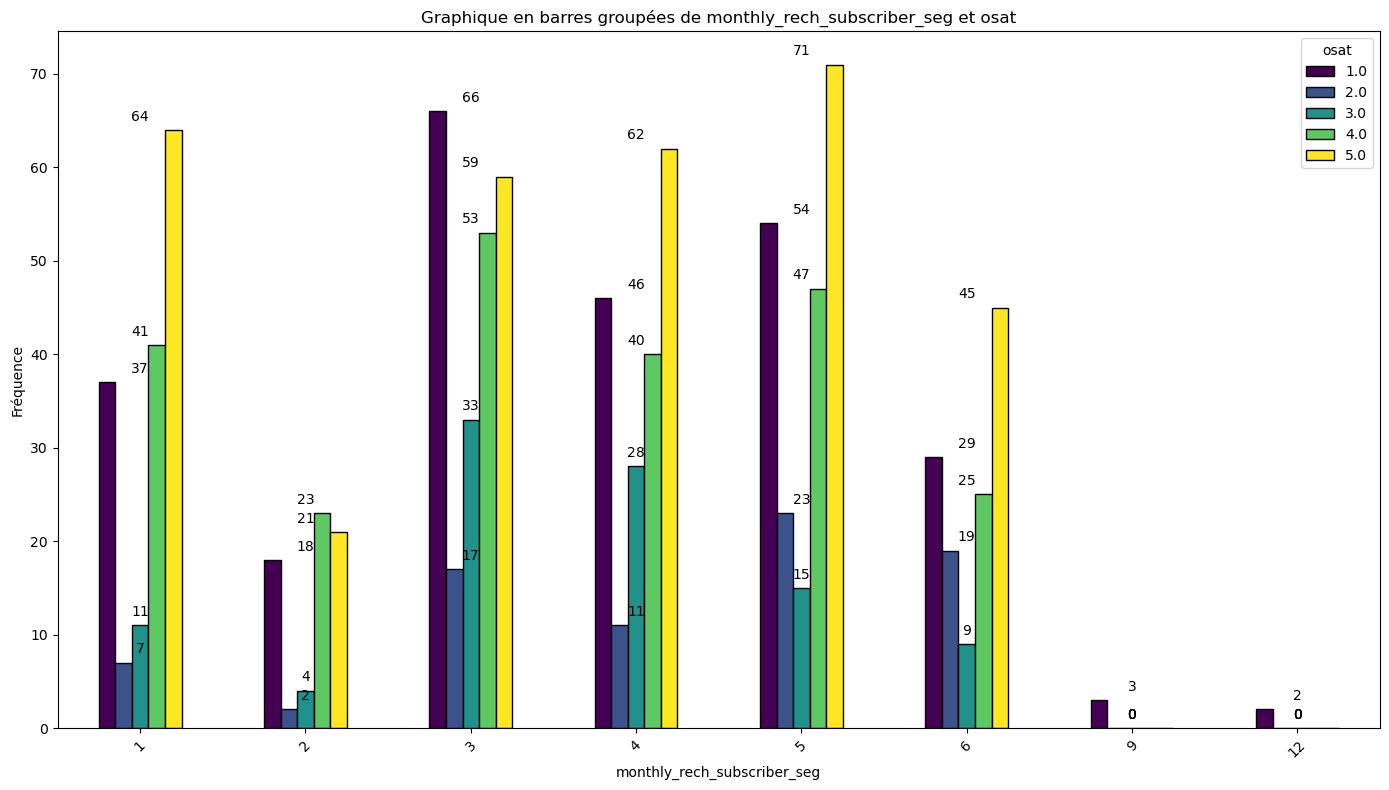
\includegraphics[width=0.7\linewidth]{barre_monthl_rech.png}
    \caption{Distribution de la variable \textbf{monthly\_rech\_subscriber\_seg} par classe \textbf{OSAT} multiclasse.}
    \label{fig:barre_monthl_rech}
\end{figure}

Comme le montre la figure \ref{fig:barre_monthl_rech}, les classes 1 et 5 sont les plus représentées dans les segments de recharge mensuelle, notamment dans les segments 1 et 6, avec une fréquence plus élevée. Les autres classes, telles que les classes 2, 3 et 4, sont moins représentées dans ces segments, ce qui indique une disparité dans les comportements de recharge des utilisateurs selon leur classe d'OSAT.

Passons maintenant à la comparaison avec \textbf{OSAT} binaire.

\begin{figure}[H]
    \centering
    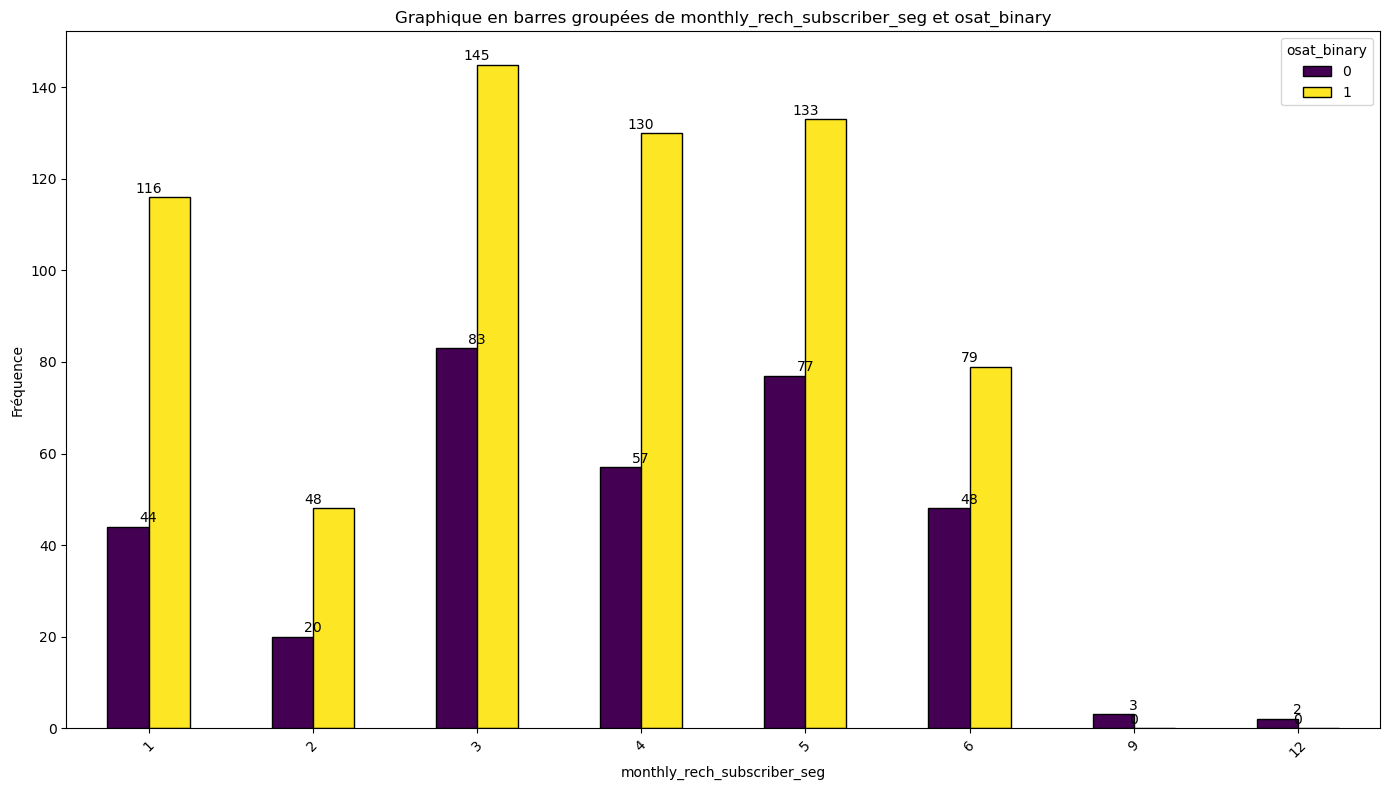
\includegraphics[width=0.7\linewidth]{barre_monthl_rech_binary.png}
    \caption{Distribution de la variable \textbf{monthly\_rech\_subscriber\_seg} par classe \textbf{OSAT} binaire.}
    \label{fig:barre_monthl_rech_binary}
\end{figure}

Dans la version binaire, comme le montre la figure \ref{fig:barre_monthl_rech_binary}, les utilisateurs satisfaits (classe 1) sont largement dominants dans tous les segments de recharge mensuelle, particulièrement dans les segments 3 et 5. À l'inverse, les utilisateurs insatisfaits (classe 0) sont moins présents, ce qui reflète un comportement de recharge moins intense pour cette classe.

\begin{figure}[H]
    \centering
    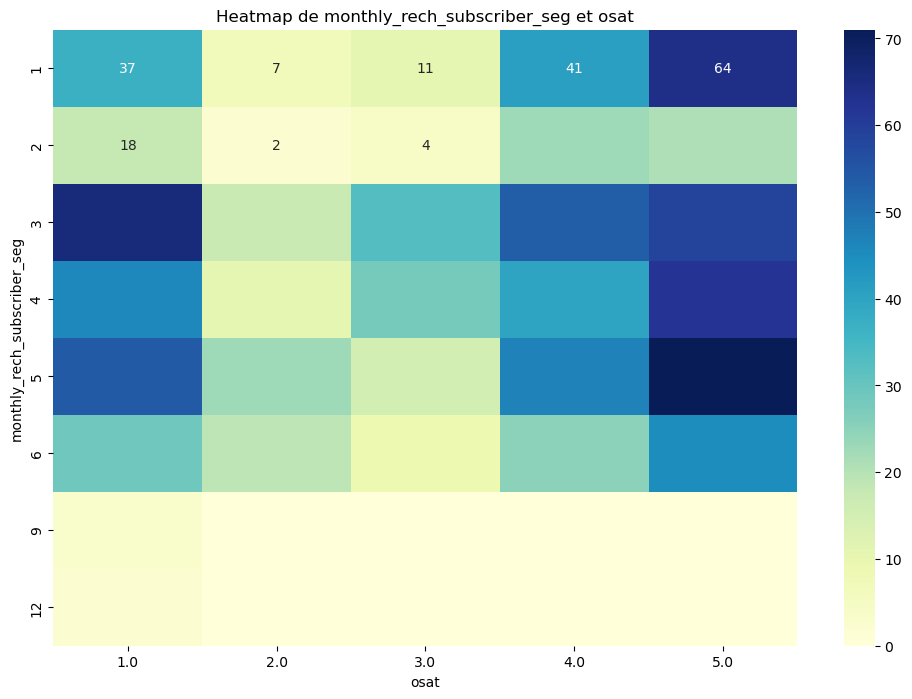
\includegraphics[width=0.7\linewidth]{heatmap_monthly_recharge.png}
    \caption{Heatmap de la variable \textbf{monthly\_rech\_subscriber\_seg} par classe \textbf{OSAT} multiclasse.}
    \label{fig:heatmap_monthly_recharge}
\end{figure}

La carte de chaleur (\ref{fig:heatmap_monthly_recharge}) met en évidence une forte concentration d'utilisateurs dans les classes 1 et 5 pour les segments 1, 5 et 6, confirmant les tendances observées dans le graphique en barres.

\begin{figure}[H]
    \centering
    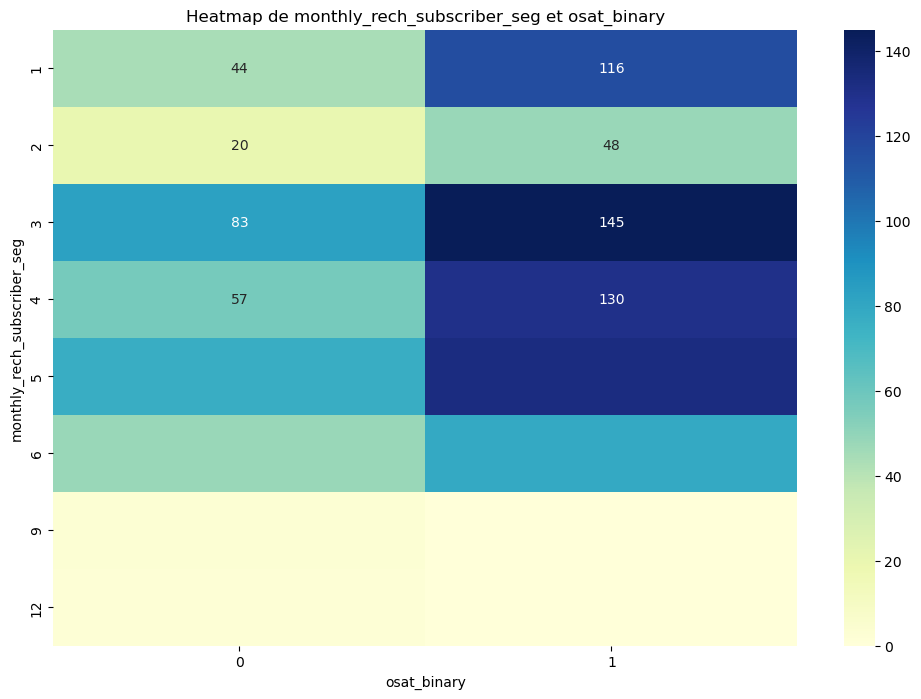
\includegraphics[width=0.7\linewidth]{heatmap_monthly_recharge_binary.png}
    \caption{Heatmap de la variable \textbf{monthly\_rech\_subscriber\_seg} par classe \textbf{OSAT} binaire.}
    \label{fig:heatmap_monthly_recharge_binary}
\end{figure}

Pour la version binaire (\ref{fig:heatmap_monthly_recharge_binary}), on observe une dominance claire des utilisateurs satisfaits (classe 1) dans presque tous les segments de recharge, particulièrement dans les segments 3 et 5, ce qui reflète une tendance similaire à celle observée dans la version multiclasse, mais avec une distinction plus marquée.

\subsubsection*{Comparaison entre les OSAT multiclasse et OSAT binaire pour la variable \textbf{monthly\_rech\_subscriber\_seg}} 
Bien que la version multiclasse de \textbf{OSAT} offre une segmentation plus fine, les tendances principales se retrouvent également dans la version binaire. La classe 1 (satisfaits) montre une fréquence plus élevée dans les segments de recharge les plus importants (3 et 5). Par conséquent, la version binaire est privilégiée pour les analyses ultérieures afin de simplifier les interprétations sans perdre d'informations significatives.

\subsubsection*{Analyse récapitulative pour les variables qualitatives}

Les variables qualitatives ont été analysées en fonction des segments \textit{OSAT multiclasse} et \textit{OSAT binaire}. Voici un aperçu des résultats pour chaque variable.

\begin{table}[H]
    \centering
    \begin{tabular}{|p{3.5cm}|p{3.5cm}|p{3.5cm}|p{3.5cm}|} 
    \hline
    \textbf{Variable} & \textbf{OSAT multiclasse} & \textbf{OSAT binaire} & \textbf{Observations générales} \\ 
    \hline
    \textit{Device Type} & 
    La classe 3 présente des valeurs élevées & 
    Les valeurs sont concentrées dans la classe 1 & 
    Segment 3 reste important dans les deux OSAT \\ 
    \hline
    \textit{Monthly ARPU Subscriber Seg} & 
    La classe 12 a des valeurs très élevées & 
    Segment 12 montre une prédominance de classe 1 & 
    Segment 12 est dominant dans les deux OSAT \\ 
    \hline
    \textit{Flag 4G Binary} & 
    Classe 1 contient la majorité des utilisateurs 4G & 
    La classe 1 reste dominante dans le segment 4G & 
    Une forte majorité est 4G dans les deux OSAT \\ 
    \hline
    \textit{Flag Smartphone} & 
    Les classes 1 et 5 montrent une grande utilisation de smartphones & 
    La majorité des utilisateurs sont dans la classe 1 & 
    Utilisation généralisée de smartphones dans les deux OSAT \\ 
    \hline
    \textit{Number of Reactivation} & 
    Classe 1 a des réactivations élevées & 
    Les réactivations sont dominées par la classe 0 & 
    Répartition similaire dans les deux OSAT \\ 
    \hline
    \end{tabular}
    \caption{Résumé des variables qualitatives entre \textit{OSAT multiclasse} et \textit{OSAT binaire}.}
\end{table}

\subsubsection*{Comparaison générale entre OSAT multiclasse et OSAT binaire pour les variables qualitatives}
La version multiclasse d'OSAT offre une segmentation plus détaillée des variables qualitatives, mais les différences entre les classes restent souvent subtiles. La version binaire simplifie l'analyse sans perte majeure d'information, facilitant ainsi l'interprétation tout en réduisant la complexité. Pour les prochaines analyses, OSAT binaire est privilégiée en raison de son efficacité et de sa clarté.

\subsubsection{Comparaison globale entre OSAT multiclasse et OSAT binaire}
L'analyse des variables quantitatives et qualitatives montre que, bien que la version multiclasse d'OSAT permette une segmentation plus fine, les différences observées entre les classes sont généralement minimes. La version binaire d'OSAT simplifie l'interprétation sans perte significative d'information. Cette simplification réduit la complexité des analyses tout en maintenant une clarté et une cohérence suffisantes dans les résultats. Par conséquent, l'utilisation d'OSAT binaire est privilégiée pour les prochaines étapes, car elle permet une analyse plus efficace et facile à interpréter.


\subsection{Analyse inférentielle}

L'objectif de l'analyse inférentielle est de comprendre les relations entre la variable cible (\textbf{OSAT}) et les différentes \textbf{features} explicatives, qu'elles soient quantitatives ou qualitatives. Dans cette section, nous explorons la corrélation entre les variables qualitatives et quantitatives, ainsi que la corrélation entre variables qualitatives elles-mêmes.
on a d'abord examiné la corrélation entre la variable cible (\textbf{OSAT}) et les différentes \textbf{features} quantitatives. L'analyse de corrélation est illustrée par une matrice de corrélation, dans laquelle on a utilisé le coefficient de corrélation de Pearson pour évaluer la relation linéaire entre les variables.
\begin{figure}[H]
    \centering
    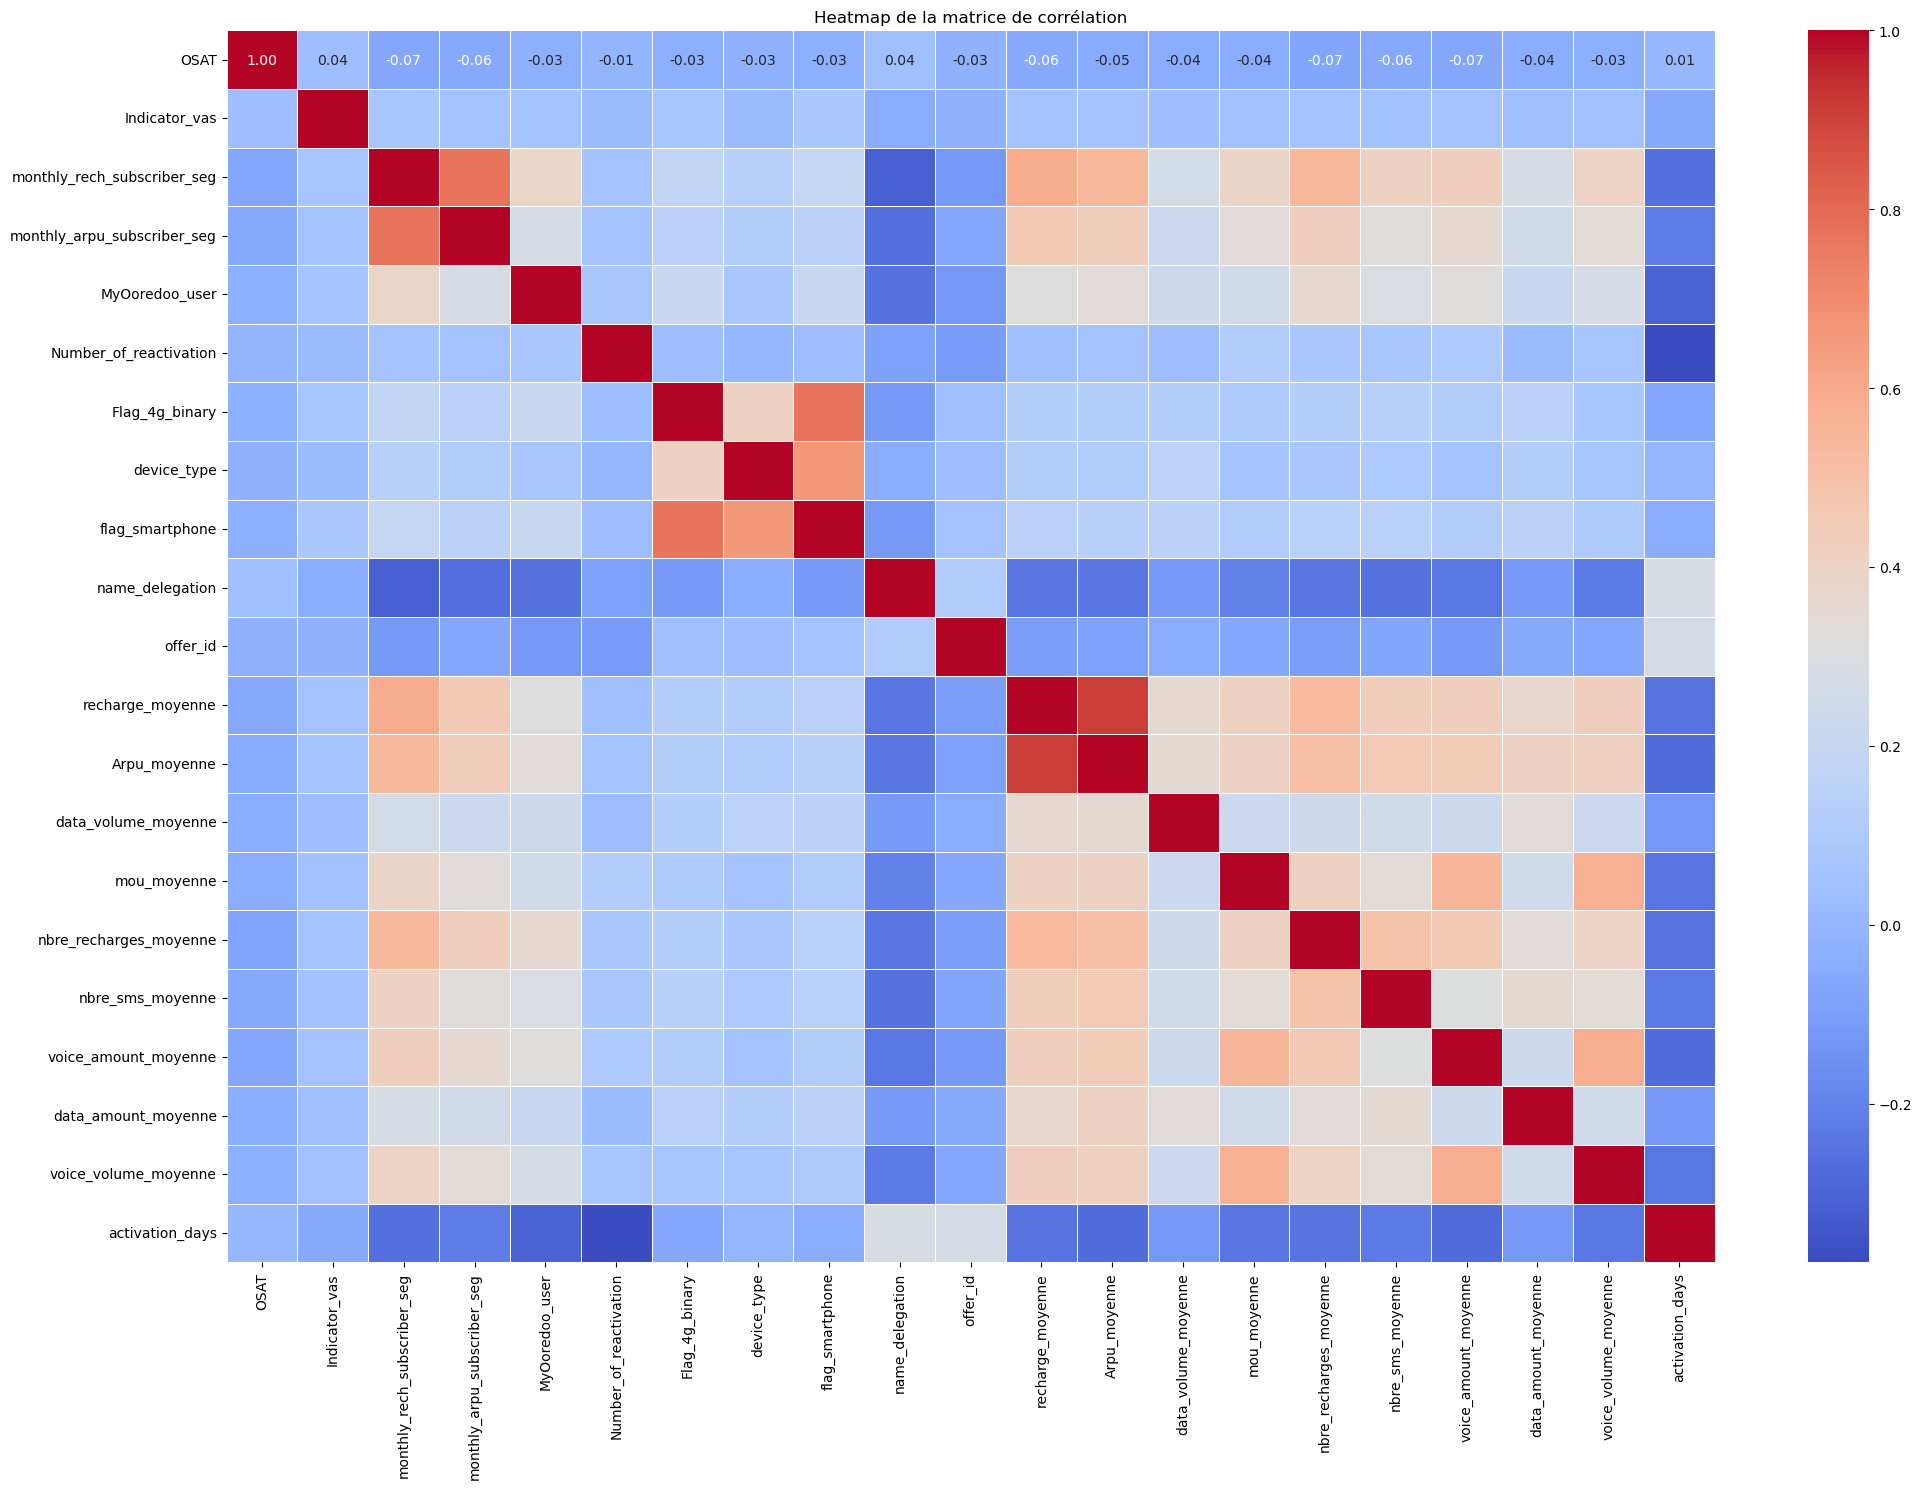
\includegraphics[width=0.7\linewidth]{Correlation_Retail.png}
    \caption{Heatmap de la matrice de corrélation globale pour la table de Juin.}
    \label{fig:correlation_matrix}
\end{figure}

\subsubsection{Corrélation entre la variable cible et les variables explicatives}
\subsubsection*{Corrélation entre les variables qualitatives et la variable cible}

Pour évaluer la relation entre des variables qualitatives comme \textbf{device\_type} et \textbf{osat}, plusieurs indicateurs statistiques ont été utilisés, notamment \textbf{Cramér's V} et le \textbf{test du Chi-Carré}, afin de mesurer et évaluer la force de leur association.

\textbf{1. Indice de Cramér’s V:} Cet indice mesure la force de l'association entre deux variables qualitatives. L'indice de Cramér’s V varie entre 0 et 1, où une valeur proche de 0 indique une faible association et une valeur proche de 1 indique une association forte.

\textit{Le code utilisé pour calculer cet indice est présenté dans l'annexe, voir Figure \ref{00}.}

\textbf{\checkmark Exemple de résultat:} Pour la relation entre \textbf{device\_type} et \textbf{osat}, un Cramér's V de \textbf{0.0297} a été obtenu, ce qui indique une association faible.

    
\textbf{2. Test du Chi-Carré:} Ce test permet de vérifier s'il existe une association statistiquement significative entre deux variables qualitatives. Si la p-value est inférieure à 0.05, cela indique une association significative.

\textit{Le code utilisé pour effectuer le test du Chi-Carré est présenté dans l'annexe, voir Figure \ref{222}.}

Pour la relation entre \textbf{device\_type} et \textbf{osat\_binary} (binarisation d'OSAT), une p-value de \textbf{0.7528} a été obtenue, indiquant qu'il n'y a pas d'association significative.

\textbf{\checkmark Exemple de tableau de contingence:}

\begin{figure}[H]
    \centering
    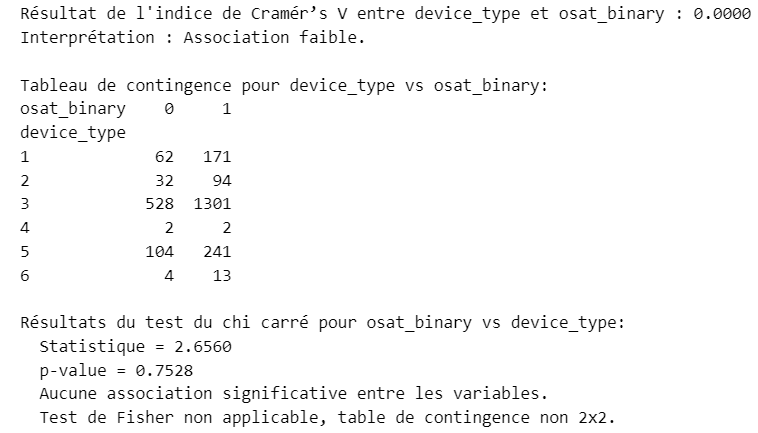
\includegraphics[width=0.6\linewidth]{capture_sas_39.png}
    \caption{Tableau de contingence pour \textbf{device\_type} et \textbf{osat\_binary}.}
\end{figure}

Le test du Chi-Carré confirme qu'il n'y a pas d'association significative entre \textbf{device\_type} et \textbf{osat\_binary} (p-value = 0.7528). Le test de Fisher n'était pas applicable, car le tableau de contingence n'était pas de dimension 2x2.

Cette méthodologie a été appliquée pour toutes les autres variables qualitatives.

\textbf{\(\rightarrow\)} \textbf{Variables avec faible association:} Certaines variables montrent une faible association avec la satisfaction (\textbf{OSAT}), notamment \textbf{monthly\_arpu\_subscriber\_seg}, \textbf{monthly\_rech\_subscriber\_seg}, \textbf{flag\_smartphone}, et \textbf{Number\_of\_reactivation}. Les indices de \textbf{Cramér's V} sont inférieurs à 0.1 et les \textbf{p-values} du \textbf{Chi-Carré} dépassent 0.05, indiquant une faible ou aucune association statistiquement significative.


\textbf{\(\rightarrow\)} \textbf{Variables sans association significative:} Les variables \textbf{Flag\_4g\_binary} et \textbf{flag\_smartphone} n’ont montré aucune association avec \textbf{osat\_binary}. Les \textbf{p-values} sont supérieures à 0.05, confirmant l'absence de relation statistiquement significative.


\textbf{\(\rightarrow\)} \textbf{Variable avec une association significative:} La variable \textbf{monthly\_rech\_subscriber\_seg} montre une association significative avec une \textbf{p-value} de \textbf{0.0211}, suggérant un impact potentiel sur la satisfaction (\textbf{osat\_binary}).

\noindent \textbf{3. Analyse de l'association par la Lambda de Goodman et Kruskal:} Pour approfondir l'analyse des relations entre les variables qualitatives et \textbf{osat\_binary}, on a calculé la \textbf{Lambda de Goodman et Kruskal}, qui évalue la réduction d'erreur dans la prédiction d'une variable en fonction d'une autre.

\textit{Le code utilisé pour calculer la Lambda de Goodman et Kruskal est présenté dans l'annexe, voir Figure \ref{555}.}

\textbf{\checkmark Exemple de résultat:} Pour la variable \textbf{Flag\_4g\_binary}, une Lambda de \textbf{0.42} a été obtenue, indiquant que la connaissance de cette variable permet une réduction d'erreur de \textbf{42\%} dans la prédiction de \textbf{osat\_binary}.

\textit{Le résultat de la Lambda de Goodman et Kruskal est présenté dans l'annexe, voir Figure \ref{AnB1}.}


\textbf{\checkmark Résultats pour les autres variables:} Les résultats montrent que \textbf{device\_type} a une lambda de 0.15, indiquant une faible réduction d'erreur, tandis que \textbf{flag\_smartphone} et \textbf{Number\_of\_reactivation} affichent des lambdas de 0.60 et 0.84 respectivement, signalant une réduction d'erreur plus significative. En revanche, \textbf{monthly\_arpu\_subscriber\_seg} et \textbf{monthly\_rech\_subscriber\_seg} n'ont aucune réduction d'erreur avec des lambdas nulles.

Cela montre que certaines variables, comme \textbf{flag\_smartphone} et \textbf{Number\_of\_reactivation}, influencent la satisfaction (\textbf{osat\_binary}), tandis que d'autres, comme \textbf{monthly\_arpu\_subscriber\_seg}, n'apportent aucune valeur prédictive.

\subsubsection*{Corrélation entre les variables quantitatives et la variable cible}

Pour évaluer la relation entre les variables quantitatives et la variable cible \textbf{osat\_binary}, on a utilisé l'indicateur de \textbf{l'Eta carré}. Cet indicateur permet de mesurer l'effet de la variable explicative sur la variable cible. Le calcul de l'Eta carré a été effectué pour \textbf{osat\_binary}.

\textit{Le code utilisé pour calculer l'Eta carré est présenté en annexe, voir Figure \ref{26203}.}

Ensuite, pour déterminer le test statistique à utiliser, on a vérifié la normalité et l'homogénéité des variances avec les tests de \textbf{Shapiro-Wilk} et \textbf{Levene}. Si les conditions étaient remplies, on a utilisé le \textbf{test t de Student}. Sinon, le \textbf{test de Mann-Whitney} a été appliqué.

\textit{Le code de ces tests est disponible en annexe, voir Figure \ref{168}.}

\textbf{Résultats pour la variable Recharge:}

Pour la variable quantitative \textbf{recharge}, l'ensemble des tests a été appliqué afin d'évaluer son association avec \textbf{OSAT}. Voici les résultats obtenus à chaque étape.

\textbf{\checkmark Résultat de l'Eta carré:} L'indicateur de \textbf{l'Eta carré} montre un effet très faible pour \textbf{OSAT}, avec une valeur de \textbf{0.0064}. 

\textit{Résultat de l'Eta carré pour osat\_binary est disponible en annexe, voir Figure \ref{AnB3}.}


L'interprétation de ce résultat indique que l'effet de la variable explicative sur la satisfaction (\textbf{OSAT}) est très faible, suggérant une influence limitée.

\textbf{\checkmark Test pour \textbf{osat\_binary}:} Les tests de \textbf{Shapiro-Wilk} montrent que les données ne suivent pas une distribution normale pour les deux groupes (statistiques de \textbf{0.7522} pour le groupe 0 et \textbf{0.6954} pour le groupe 1, avec des p-values inférieures à 0.05). De plus, le test de \textbf{Levene} indique que les variances ne sont pas homogènes (\textbf{p-value = 0.0273}). Par conséquent, les conditions pour appliquer un test paramétrique ne sont pas respectées. Nous avons donc appliqué le \textbf{test de Mann-Whitney}, qui révèle des différences significatives entre les deux groupes (\textbf{p-value = 0.0003}). 


\textit{Les résultats du test de normalité et de variances et du test de Mann-Whitney sont disponibles en annexe, voir Figure \ref{AnB4} et \ref{AnB5}.}



Les résultats du test de Mann-Whitney montrent une différence significative entre les distributions de la variable \textbf{recharge\_moyenne} pour les deux groupes de \textbf{osat\_binary} (\textbf{p-value = 0.0003}), indiquant que les valeurs de \textbf{recharge\_moyenne} diffèrent significativement selon les niveaux de \textbf{osat\_binary}.

Pour \textbf{osat multiclasse}, les tests ont montré des résultats similaires avec des différences significatives entre les groupes (p-value = 0.0003).

\textbf{Conclusion des tests:} Les tests de normalité (\textbf{Shapiro-Wilk}) et d'homogénéité des variances (\textbf{Levene}) n'ont pas été vérifiés pour les variables quantitatives étudiées. Par exemple, pour \textbf{Arpu}, le test de Shapiro-Wilk a donné des p-values de \textbf{0.0000}, indiquant une distribution non normale. Bien que certaines variables, comme \textbf{Arpu}, aient montré des variances homogènes (p = \textbf{0.0801}), les conditions d'application des tests paramétriques n'ont globalement pas été respectées.

En conséquence, tous les tests utilisés sont non paramétriques : le \textbf{Mann-Whitney} pour \textbf{osat\_binary} et le \textbf{Kruskal-Wallis} pour \textbf{OSAT}. Lorsque des différences significatives ont été détectées avec Kruskal-Wallis, des comparaisons post-hoc ont été effectuées avec le test de \textbf{Dunn}. Le tableau ci-dessous résume les résultats :

\begin{longtable}{|l|c|c|c|p{3cm}|}
\hline
\textbf{Variable} & \textbf{Eta carré} & \textbf{Test U (osat\_binary)} & \textbf{Kruskal-Wallis (osat)} &  \textbf{Interprétation finale} \\ 
\hline
\textbf{Arpu} & 0.0057 & p = 0.0005 & p = 0.0011 & Différences significatives \\ 
\hline
\textbf{Voice volume} & 0.0047 & p = 0.0008 & p = 0.0001  & Différences significatives \\ 
\hline
\textbf{Voice amount} & 0.0078 & p = 0.0001 & p = 0.0001  & Différences significatives \\ 
\hline
\textbf{Data volume} & 0.0029 & p = 0.1979 & p = 0.2741  & Pas de différences significatives \\ 
\hline
\textbf{Mou} & 0.0042 & p = 0.0003 & p = 0.0002  & Différences significatives \\ 
\hline
\textbf{Nbre of SMS} & 0.0058 & p = 0.0038 & p = 0.0054 & Différences significatives \\ 
\hline
\textbf{Activation days} & - & p = 0.8498 & p = 0.6350  & Pas de différences significatives \\ 
\hline
\end{longtable}

\subsubsection*{Conclusion }
Bien que certaines variables quantitatives et qualitatives montrent une relation avec la satisfaction (\textbf{OSAT}), la majorité d'entre elles n'indiquent pas de différences significatives. Ces résultats mettent en évidence des impacts limités des variables étudiées sur la satisfaction client.
\textbf{Variables quantitatives:} Les variables quantitatives, comme \textbf{Arpu}, \textbf{Voice Volume}, et \textbf{Mou}, montrent des différences significatives entre les groupes \textbf{OSAT}. Cependant, d'autres variables, comme \textbf{Data Volume} et \textbf{Activation days}, ne présentent pas de différences significatives.

\textbf{Variables qualitatives:} Certaines variables qualitatives, telles que \textbf{Device Type} et \textbf{Flag\_4G}, influencent significativement la satisfaction client. Toutefois, plusieurs autres, comme les segments de recharge ou d'ARPU mensuel, n'ont pas d'association significative.

\subsubsection{Analyse des corrélations entre les variables explicatives}
\subsubsection*{Variable quantitative VS Variable quantitative:}
L'analyse des corrélations entre les variables explicatives permet de détecter des redondances ou interdépendances. Une forte corrélation pourrait indiquer que deux variables véhiculent des informations similaires, ce qui peut influencer la modélisation ou l'interprétation des résultats.

Pour cela, on a utilisé à la fois des outils graphiques et des tests statistiques pour explorer la force des relations entre les variables.

\textit{Le code utilisé pour effectuer ces analyses est disponible en annexe, voir Figures \ref{molka} et \ref{hamma}.}

Le code analyse les corrélations entre deux variables explicatives. La \textbf{covariance} est calculée pour déterminer la direction de la relation (positive, négative ou inexistante). Les \textbf{tests de normalité} (Shapiro-Wilk) permettent de guider le choix entre le \textbf{test de Pearson} (corrélation linéaire pour les variables normales) et le \textbf{test de Spearman} (corrélation monotone pour les données non normales).

De plus, le code génère des \textbf{diagrammes de dispersion} qui permettent de visualiser et d'interpréter la relation en termes de force et de direction.

Cette approche permet d'explorer les relations linéaires et non linéaires, même lorsque les conditions paramétriques ne sont pas respectées.


\begin{figure}[H]
    \centering
    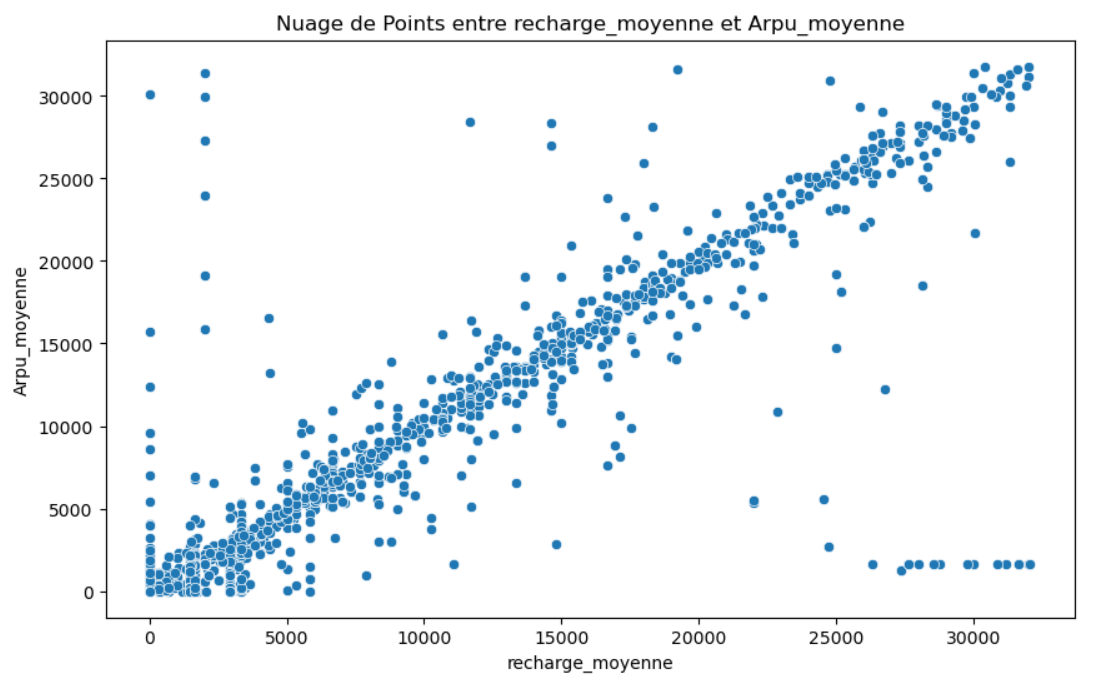
\includegraphics[width=0.6\linewidth]{capture_sas_47.png}
    \caption{Nuage de points entre \textbf{recharge\_moyenne} et \textbf{Arpu\_moyenne}}
    \label{nuage1}
\end{figure}

\noindent
Cette première figure \ref{nuage1} représente un nuage de points entre les variables \textbf{recharge\_moyenne} et \textbf{Arpu\_moyenne}. On observe une tendance positive forte, où les deux variables semblent évoluer ensemble. Cela suggère une corrélation significative.

\begin{figure}[H]
    \centering
    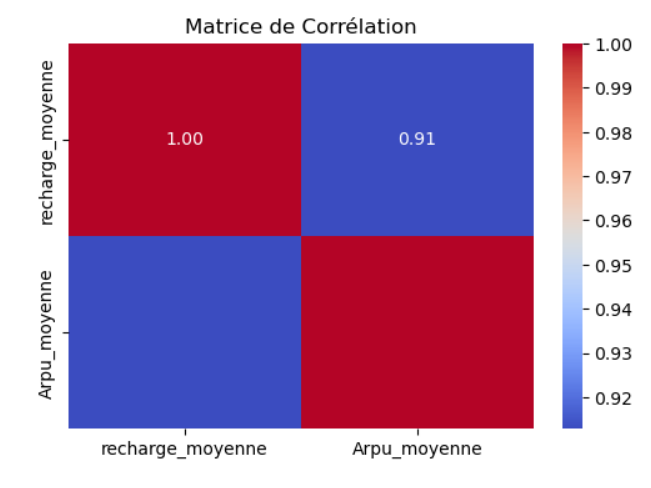
\includegraphics[width=0.5\linewidth]{capture_sas_48.png}
    \caption{Matrice de corrélation entre \textbf{recharge\_moyenne} et \textbf{Arpu\_moyenne}}
    \label{matrice1}
\end{figure}

\noindent
La matrice de corrélation dans la figure \ref{matrice1} confirme cette observation avec un coefficient de corrélation de \(0.91\), indiquant une corrélation forte et positive entre ces deux variables.\par

\textit{La figure \ref{11} de l'annexe B résume les résultats de la covariance, des tests de normalité, et du test de corrélation entre les variables \textbf{recharge\_moyenne} et \textbf{Arpu\_moyenne}. Comme les deux variables ne suivent pas une distribution normale, on a utilisé le test non paramétrique de Spearman pour évaluer la corrélation.}



\noindent
Le test de Shapiro-Wilk a montré que les deux variables \textbf{recharge\_moyenne} et \textbf{Arpu\_moyenne} ne suivent pas une distribution normale, avec des p-values très faibles (inférieures à 0.05). Par conséquent, le test non paramétrique de Spearman a été utilisé, et il a révélé une corrélation positive et forte entre ces deux variables (\textbf{r = 0.9450}, \textbf{p-value = 0.0000}). Cela signifie que lorsque \textbf{recharge\_moyenne} augmente, \textbf{Arpu\_moyenne} tend également à augmenter.

\begin{figure}[H]
    \centering
    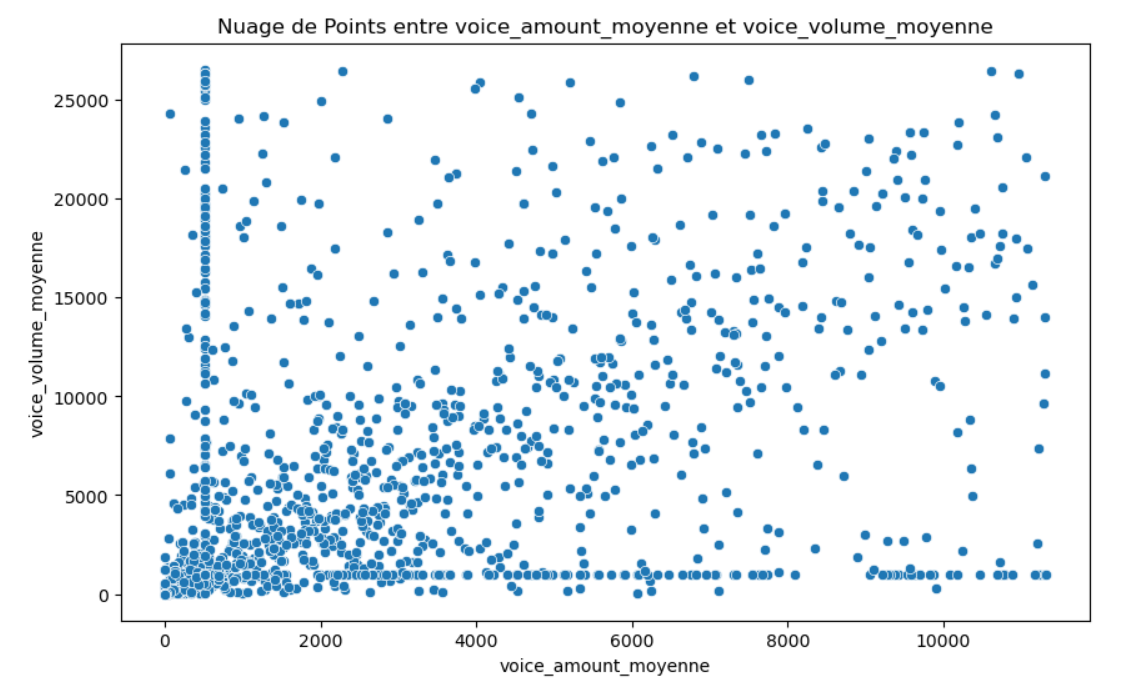
\includegraphics[width=0.6\linewidth]{capture_sas_50.png}
    \caption{Nuage de points entre \textbf{voice\_volume\_moyenne} et \textbf{voice\_amount\_moyenne}}
    \label{nuage4}
\end{figure}

\noindent
La figure \ref{nuage4} montre un nuage de points entre les variables \textbf{voice\_volume\_moyenne} et \textbf{voice\_amount\_moyenne}. Bien que la tendance soit visible, la relation reste modérée.

\begin{figure}[H]
    \centering
    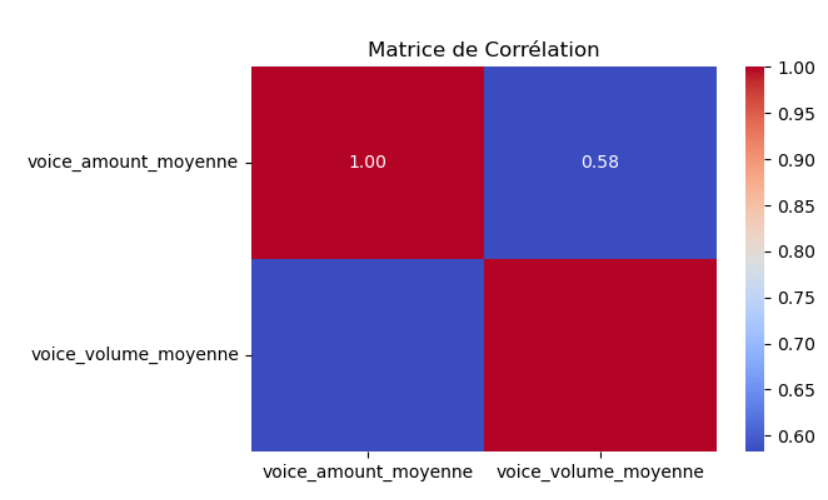
\includegraphics[width=0.5\linewidth]{capture_sas_51.png}
    \caption{Matrice de corrélation entre \textbf{voice\_volume\_moyenne} et \textbf{voice\_amount\_moyenne}}
    \label{matrice4}
\end{figure}

\noindent
La matrice de corrélation dans la figure \ref{matrice4} montre un coefficient de corrélation de \(0.58\), ce qui suggère une relation modérée entre ces deux variables.

\noindent
Les résultats des tests de Shapiro-Wilk montrent que les deux variables ne suivent pas une distribution normale, avec des p-values inférieures à 0.05. Le test de Spearman a révélé une corrélation modérée mais significative (\textbf{r = 0.58}, \textbf{p-value = 0.0000}). Cela indique que les deux variables ont tendance à augmenter ensemble, bien que la relation soit modérée.

\subsubsection*{Conclusion }

Les résultats de l'analyse des corrélations révèlent que plusieurs variables quantitatives présentent des relations significatives. Par exemple, la corrélation entre \textbf{recharge moyenne} et \textbf{ARPU} est forte avec un coefficient de \(r = 0.91\), ce qui suggère qu'une augmentation de la recharge moyenne est associée à une augmentation de l'ARPU. De même, la \textbf{voice\_volume\_moyenne} et la \textbf{voice\_amount\_moyenne} montrent également une corrélation positive avec \(r = 0.58\), reflétant une relation modérée entre ces deux variables.

En revanche, certaines relations, comme entre \textbf{recharge moyenne} et \textbf{activation\_days}, affichent une corrélation négative et faible (\(r = -0.25\)), suggérant une tendance inverse entre l'ancienneté du client et la fréquence des recharges. D'autres variables, telles que \textbf{nbre\_sms\_moyenne} et \textbf{recharge\_moyenne}, présentent une corrélation positive modérée (\(r = 0.77\)).

Globalement, les corrélations entre les variables de consommation, comme la \textbf{mou moyenne} ou le \textbf{data volume}, sont souvent positives et significatives, tandis que certaines variables temporelles ou d'ancienneté montrent un impact moins direct ou négatif.

\textbf{2. Variable quantitative VS Variable qualitative:}

on va maintenant analyser les corrélations entre les variables explicatives quantitatives et qualitatives afin de comprendre leur interdépendance et leur impact potentiel sur les résultats.

Pour cette section, nous analysons les relations entre les variables explicatives quantitatives et qualitatives en utilisant les tests ANOVA et Kruskal-Wallis. Voici un exemple illustré par la figure ci-dessous.

\begin{figure}[H]
    \centering
    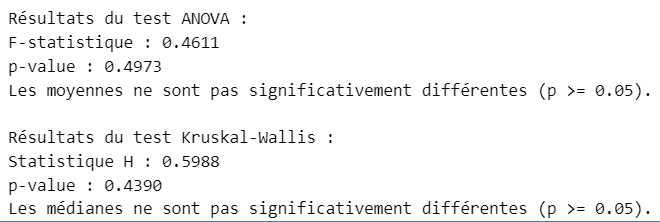
\includegraphics[width=0.7\linewidth]{capture_sas_36.png}
    \caption{Tests ANOVA/Kruskal-Wallis entre \textbf{mou\_moyenne} et \textbf{Flag\_4g\_binary}}
    \label{flag4g_mou}
\end{figure}

La figure \ref{flag4g_mou} présente l'analyse de \textbf{mou\_moyenne} selon la variable qualitative \textbf{Flag\_4g\_binary}. Les résultats des tests ANOVA et Kruskal-Wallis montrent des différences significatives entre les groupes (\textbf{p-value} < 0.05), indiquant que les utilisateurs du \textbf{Flag 4G} consomment significativement plus de minutes (\textbf{mou\_moyenne}) que les non-utilisateurs.

Dans cet exemple, nous observons que l'accès à la 4G semble être associé à une augmentation de la consommation de minutes, ce qui suggère une corrélation significative entre ces variables.

\subsection*{Conclusion }
Pour le reste des analyses, on a appliqué la même méthodologie aux différentes combinaisons de variables quantitatives et qualitatives. Voici quelques exemples de résultats obtenus:

\begin{itemize}
    \item \textbf{activation\_days} vs \textbf{flag\_smartphone}: différences significatives (ANOVA p-value = 0.0232, Kruskal-Wallis p-value = 0.0006), indiquant que la durée d'activation varie selon l'utilisation du smartphone.
    \item \textbf{recharge\_moyenne} vs \textbf{Number\_of\_reactivation}: différences significatives (ANOVA p-value = 0.0164, Kruskal-Wallis p-value = 0.0000), avec une moyenne de recharge plus élevée pour les utilisateurs ayant des réactivations.
    \item \textbf{mou\_moyenne} vs \textbf{Number\_of\_reactivation}: différences très significatives (ANOVA p-value = 0.0000, Kruskal-Wallis p-value = 0.0000), montrant une consommation plus importante de minutes pour les utilisateurs réactivés.
    \item \textbf{nbre\_recharges\_moyenne} vs \textbf{Number\_of\_reactivation}: différences significatives (ANOVA p-value = 0.0000, Kruskal-Wallis p-value = 0.0000), les utilisateurs réactivés ayant un nombre moyen de recharges plus élevé.
\end{itemize}

Ces analyses montrent que des variables qualitatives comme \textbf{flag\_smartphone} et \textbf{Number\_of\_reactivation} sont significativement associées à des variables quantitatives telles que \textbf{mou\_moyenne} et \textbf{recharge\_moyenne}, suggérant leur importance pour les futurs modèles.

% \subsubsection{Visualisation Tridimensionnelle des Relations}

% Cette section explore les relations entre les variables continues (\textbf{recharge\_moyenne}, \textbf{Arpu\_moyenne}, \textbf{mou\_moyenne}, \textbf{nbre\_sms\_moyenne}) et la variable qualitative \textbf{OSAT}, à travers des visualisations tridimensionnelles qui clarifient leur influence sur la satisfaction.


% \begin{figure}[H]
%     \centering
%     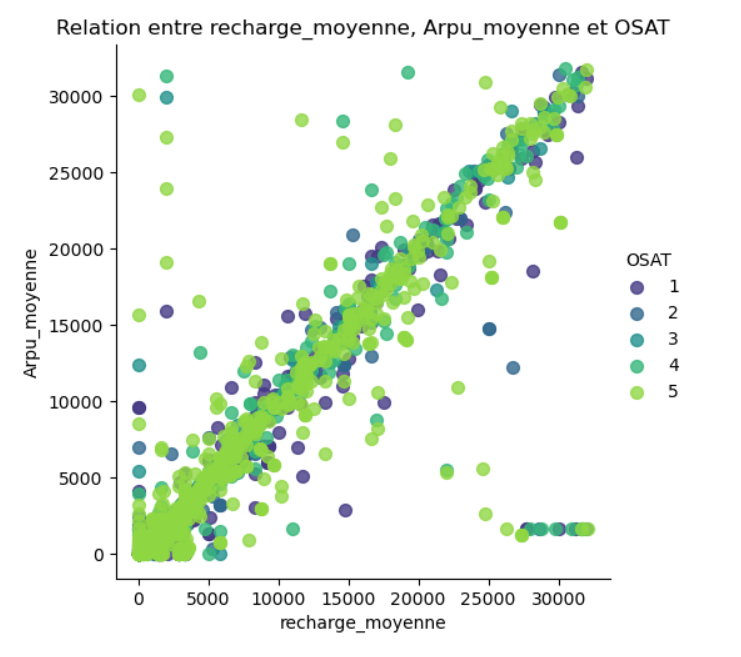
\includegraphics[width=0.5\linewidth]{capture_sas_54.png}
%     \caption{Relation entre \textbf{recharge\_moyenne}, \textbf{Arpu\_moyenne} et \textbf{osat}}
%     \label{22}
% \end{figure}

% La figure \ref{22} montre une relation positive entre \textbf{recharge\_moyenne} et \textbf{Arpu\_moyenne}, suggérant que l'augmentation des recharges est liée à une hausse de l'ARPU. Les niveaux de satisfaction (\textbf{OSAT}) révèlent une tendance où des recharges plus élevées correspondent souvent à une meilleure satisfaction (OSAT=4 ou 5). 

% Cependant, des clients avec un faible OSAT (1 ou 2) peuvent aussi avoir des recharges élevées, indiquant qu'il n'y a pas de lien systématique entre recharges élevées et satisfaction.

% \begin{figure}[H]
%     \centering
%     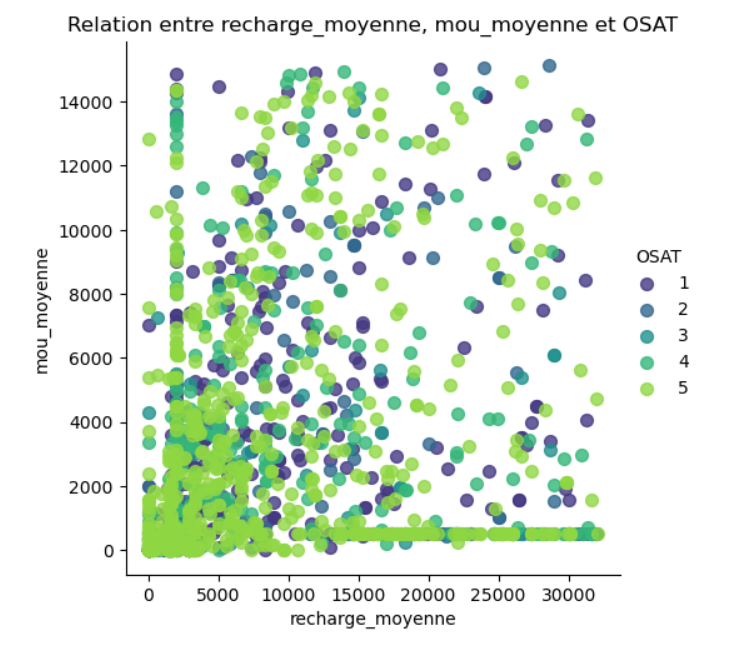
\includegraphics[width=0.5\linewidth]{capture_sas_55.png}
%     \caption{Relation entre \textbf{recharge\_moyenne}, \textbf{mou\_moyenne} et \textbf{OSAT}}
%     \label{33}
% \end{figure}

% La figure \ref{33} illustre la relation entre \textbf{recharge\_moyenne}, \textbf{mou\_moyenne} et les niveaux d'OSAT. 

% Contrairement à la forte corrélation observée dans le cas de \textbf{Arpu\_moyenne}, ici la relation entre \textbf{recharge\_moyenne} et \textbf{mou\_moyenne} est plus dispersée. Bien qu'il existe une légère tendance à l'augmentation de \textbf{mou\_moyenne} avec la hausse de \textbf{recharge\_moyenne}, cette relation n'est pas aussi marquée.

% Les niveaux de satisfaction (\textbf{OSAT}) varient également de manière irrégulière, sans tendance évidente ou forte séparation entre les différents groupes d'OSAT. Cela suggère que la variable \textbf{mou\_moyenne} n'a pas une influence directe sur le niveau de satisfaction, contrairement à d'autres variables comme \textbf{Arpu\_moyenne}.
% \subsubsection*{Relation entre \textbf{recharge\_moyenne}, \textbf{nbre\_sms\_moyenne} et \textbf{OSAT}}
% \begin{figure}[H]
%     \centering
%     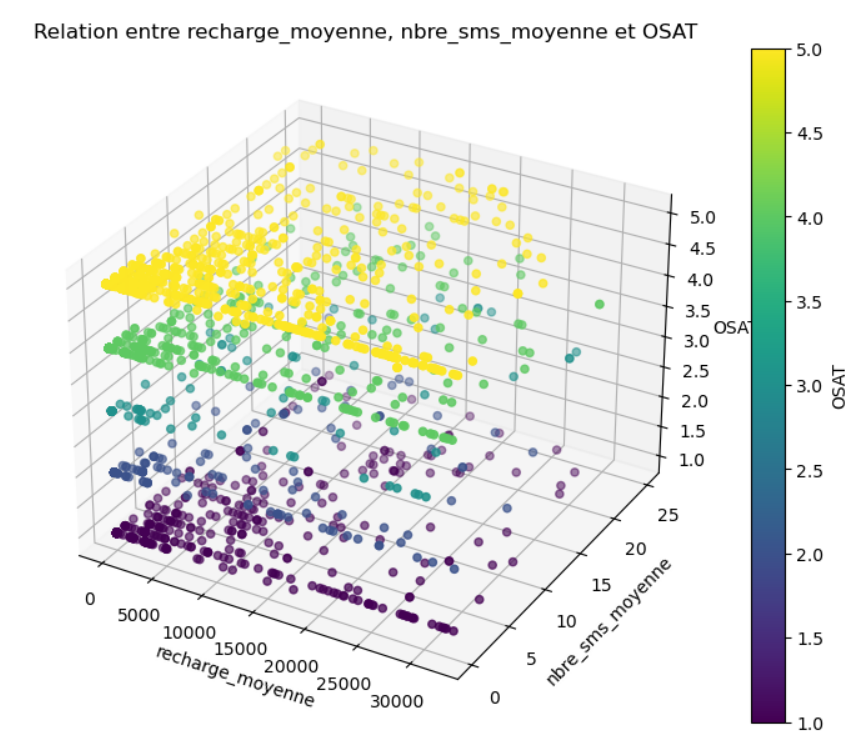
\includegraphics[width=0.6\linewidth]{capture_sas_56.png}
%     \caption{Relation entre \textbf{recharge\_moyenne}, \textbf{nbre\_sms\_moyenne} et \textbf{OSAT}}
% \end{figure}

% Cette visualisation 3D présente la relation entre \textbf{recharge\_moyenne}, \textbf{nbre\_sms\_moyenne} et \textbf{OSAT}. 

% Nous observons une légère tendance à l'augmentation des valeurs de \textbf{recharge\_moyenne} et \textbf{nbre\_sms\_moyenne}, avec une répartition ariée des niveaux de satisfaction (\textbf{OSAT}). Les utilisateurs avec un \textbf{OSAT} plus élevé semblent se concentrer dans des zones de forte \textbf{recharge\_moyenne}, tandis que les valeurs plus faibles d'\textbf{OSAT} sont davantage réparties.

% Cette visualisation tridimensionnelle permet d'explorer plus en profondeur les interactions complexes entre plusieurs variables continues et la satisfaction des utilisateurs (\textbf{OSAT}). Elle met en évidence les variables qui influencent potentiellement la satisfaction des utilisateurs, offrant ainsi des pistes d'analyse supplémentaires.

\section{Modélisation}
\subsection{Équilibrage des classes (SMOTE)}

L'équilibrage des classes de la variable cible \textbf{OSAT} a été effectué avec la méthode SMOTE (Synthetic Minority Over-sampling Technique) pour corriger la répartition initiale déséquilibrée, comme illustré par la figure \ref{smote_avant}.

\begin{figure}[H]
    \centering
    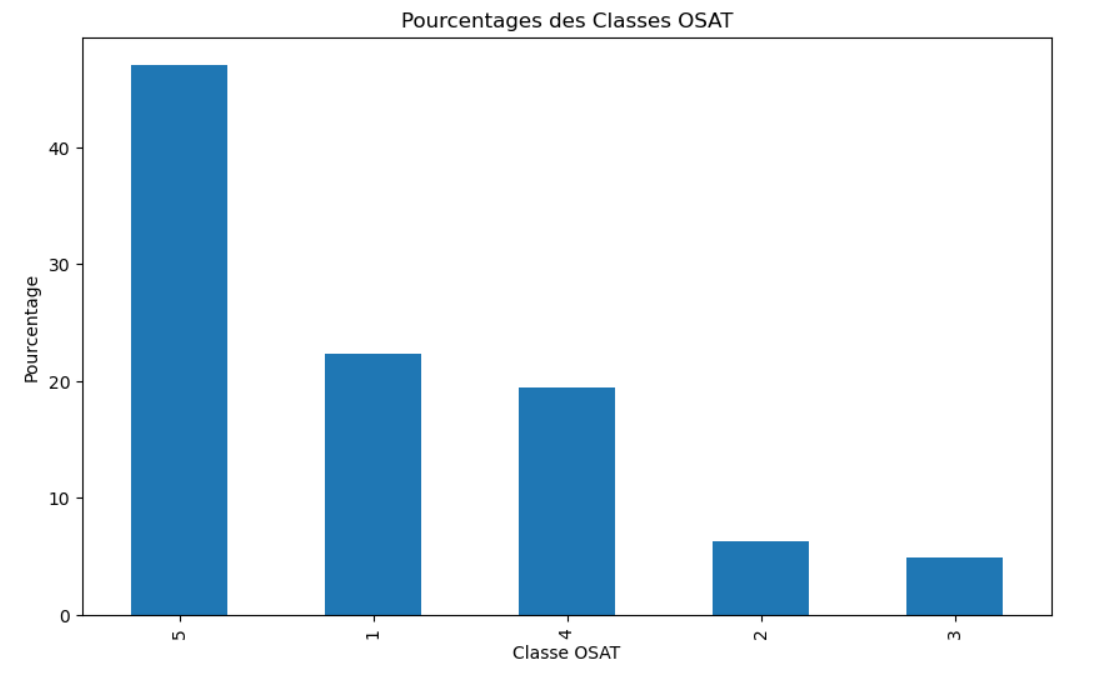
\includegraphics[width=0.7\linewidth]{capture_sas_57.png}
    \caption{Pourcentages des classes OSAT avant équilibrage}
    \label{smote_avant}
\end{figure}

Avant SMOTE, la classe 5 dominait avec 47\%, tandis que les classes 2 et 3 étaient sous-représentées. SMOTE a permis de rééquilibrer les classes en augmentant la présence des classes moins fréquentes sans suréchantillonner excessivement certaines classes.

\begin{figure}[H]
    \centering
    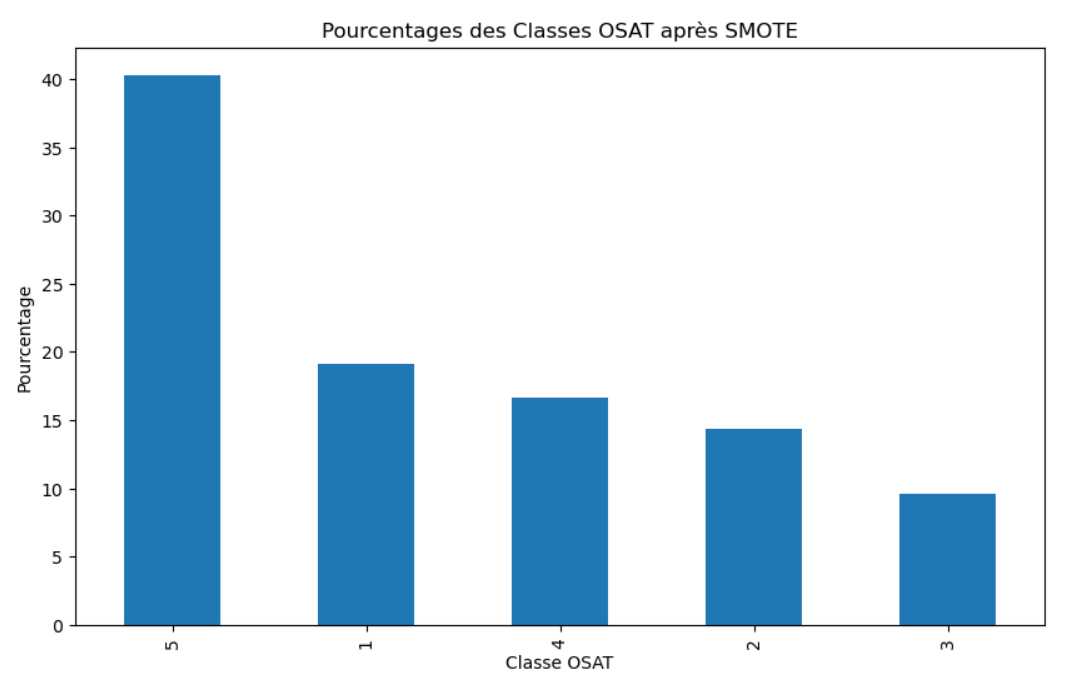
\includegraphics[width=0.7\linewidth]{capture_sas_59.png}
    \caption{Pourcentages des classes OSAT après équilibrage avec SMOTE}
    \label{smote_aprés}
\end{figure}

Après SMOTE (figure \ref{smote_aprés}), les classes sont réparties de façon plus homogène, réduisant le biais en faveur des classes majoritaires et améliorant la modélisation. Les nouvelles proportions sont :

\textbf{Classe 5}: 40.28\%, \textbf{Classe 1}: 19.15\%, \textbf{Classe 4}: 16.63\%, \textbf{Classe 2}: 14.35\%, \textbf{Classe 3}: 9.56\%.

Cette répartition équilibrée permet un jeu de données plus adapté à la modélisation et à une meilleure interprétation des résultats finaux.

\subsection{Sélection des caractéristiques}
Trois méthodes ont été appliquées pour la sélection des caractéristiques : \textbf{RFE (Recursive Feature Elimination)}, \textbf{SelectKBest}, et les \textbf{importances des caractéristiques à partir de Random Forest}. Ces méthodes permettent d'identifier les variables explicatives ayant le plus grand impact sur la prédiction de la variable cible \textbf{OSAT}. 

\textit{Le code utilisé pour effectuer cette sélection est disponible en annexe, voir Figure \ref{code_features_Selection}.}

\textbf{RFE :} La méthode RFE avec un classificateur Random Forest a identifié \textbf{recharge\_moyenne}, \textbf{data\_amount\_moyenne}, et \textbf{voice\_amount\_moyenne} comme les variables les plus pertinentes (rang 1). 

\begin{figure}[H]
    \centering
    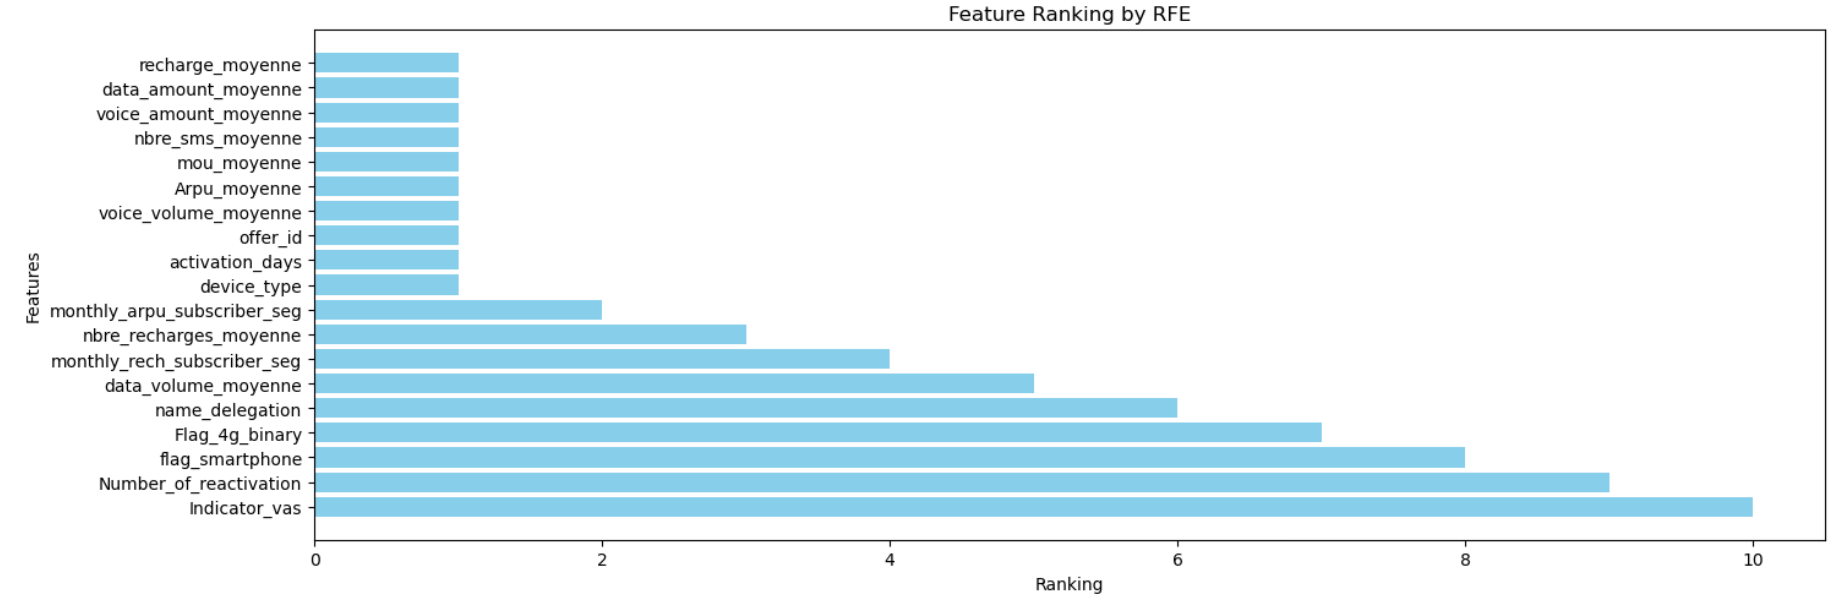
\includegraphics[width=0.8\linewidth]{capture_sas_65.png}
    \caption{Classement des caractéristiques par RFE}
\end{figure}

\textbf{SelectKBest :} Cette méthode a sélectionné des variables en fonction de leur variance expliquée. Les variables les plus influentes sont \textbf{flag\_smartphone} (score de 7.21), \textbf{recharge\_moyenne} (6.39), et \textbf{data\_amount\_moyenne} (6.38). D'autres variables importantes incluent :
\textbf{Flag\_4g\_binary} (6.12), \textbf{Arpu\_moyenne} (5.61), \textbf{voice\_volume\_moyenne} (5.43), et \textbf{monthly\_arpu\_subscriber\_seg} (5.23).

\begin{figure}[H]
    \centering
    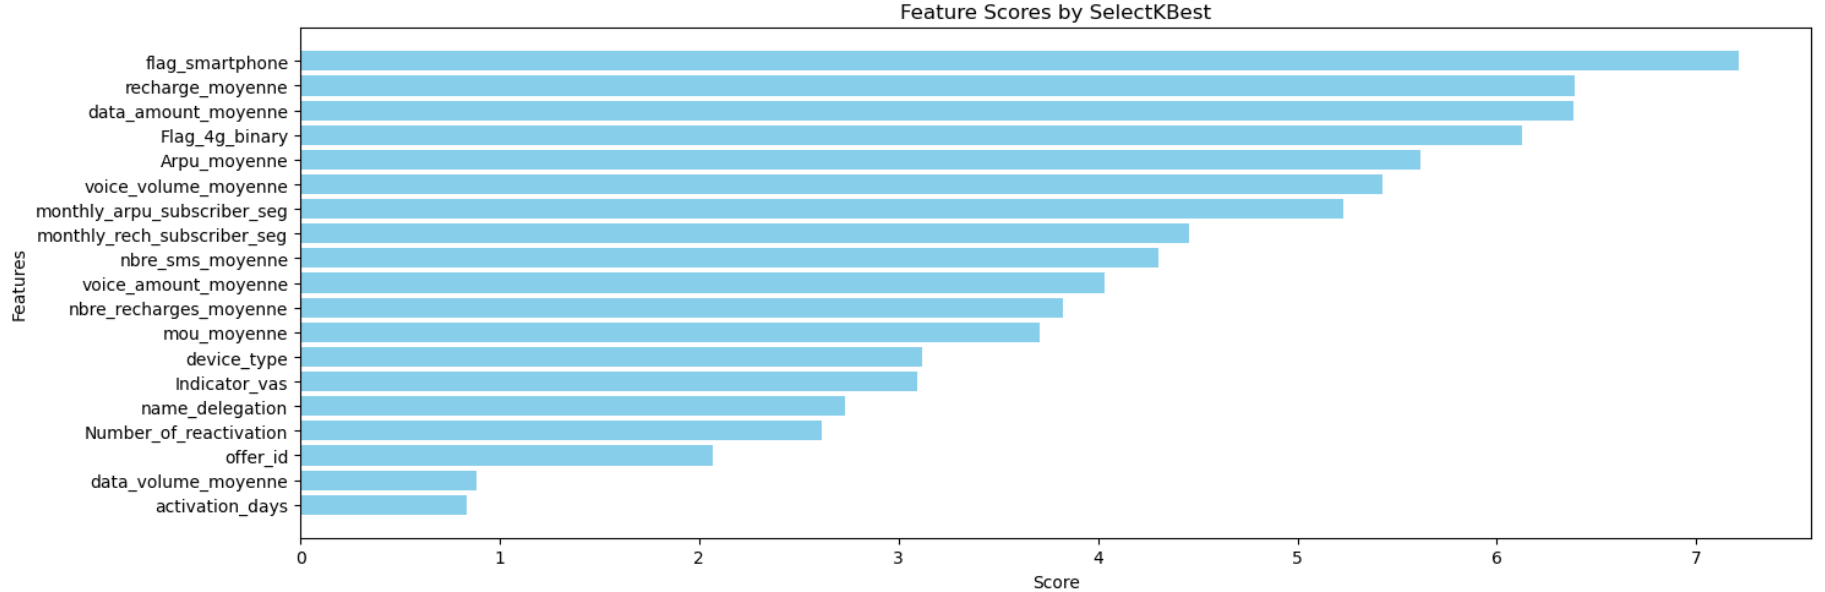
\includegraphics[width=0.8\linewidth]{capture_sas_66.png}
    \caption{Scores des caractéristiques par SelectKBest}
\end{figure}

\textbf{Random Forest :} L'analyse d'importance des caractéristiques a révélé que \textbf{activation\_days} (0.29) est la variable la plus influente, suivie par \textbf{offer\_id} (0.086) et \textbf{voice\_volume\_moyenne} (0.075). Les autres variables importantes incluent \textbf{voice\_amount\_moyenne} (0.071), \textbf{Arpu\_moyenne} (0.061), \textbf{recharge\_moyenne} (0.061), \textbf{mou\_moyenne} (0.058), et \textbf{data\_amount\_moyenne} (0.044).

\begin{figure}[H]
    \centering
    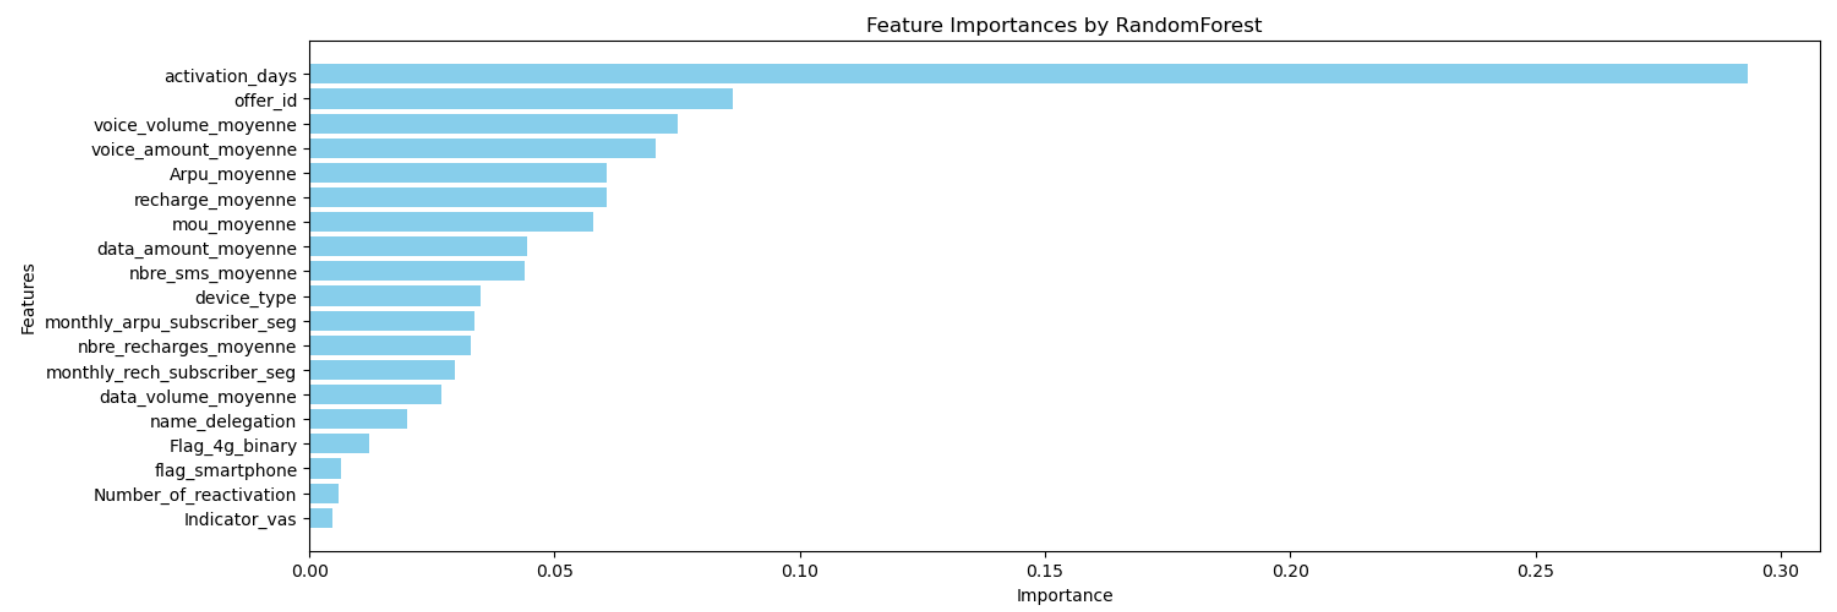
\includegraphics[width=0.8\linewidth]{capture_sas_67.png}
    \caption{Importances des caractéristiques par Random Forest}
\end{figure}


\subsubsection*{Conclusion:}
Les méthodes de sélection des caractéristiques \textbf{RFE}, \textbf{SelectKBest}, et \textbf{Random Forest} ont permis d'identifier les variables clés pour la prédiction de \textbf{OSAT}. La figure suivante montre les caractéristiques communes aux trois méthodes, telles que \textbf{recharge\_moyenne}, \textbf{voice\_amount\_moyenne}, \textbf{mou\_moyenne}, et \textbf{activation\_days}, qui se distinguent systématiquement.

\begin{figure}[H]
    \centering
    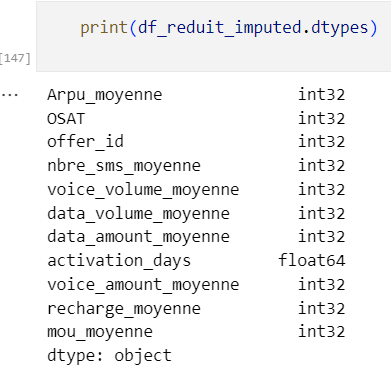
\includegraphics[width=0.4\linewidth]{capture_sas_69.png}
    \caption{Caractéristiques communes importantes entre les trois méthodes}
\end{figure}

Ce processus rigoureux a permis de définir les variables ayant un impact direct et significatif sur \textbf{OSAT}. Ces caractéristiques seront prioritaires dans les futurs modèles prédictifs pour garantir des performances optimales et des résultats fiables.

\subsection{Modélisation avec Machine Learning}

\subsubsection{Introduction}
Bien que plusieurs modèles aient été testés, cette section se concentre sur l'algorithme \textbf{Random Forest}, qui a donné les meilleurs résultats. Nous avons appliqué une validation croisée, ajusté les hyperparamètres, et évalué le modèle avec des métriques telles que l'exactitude, le rappel et la courbe ROC.

\subsubsection{Prétraitement des données}
Le prétraitement a consisté à standardiser les caractéristiques avec un \textbf{StandardScaler} pour assurer une échelle comparable entre les variables. Les données ont ensuite été divisées en ensembles d'entraînement et de test (70/30) avec \textbf{train\_test\_split}.

\subsubsection{Optimisation des hyperparamètres}
L'optimisation des hyperparamètres a été réalisée avec \textbf{RandomizedSearchCV} pour explorer efficacement différentes combinaisons de paramètres, incluant \textbf{n\_estimators}, \textbf{max\_depth}, \textbf{min\_samples\_split}, \textbf{min\_samples\_leaf}, et \textbf{criterion} (\textbf{gini} ou \textbf{entropy}). Une validation croisée à 3 plis a été utilisée pour évaluer les performances.

\textit{Le code utilisé pour l'optimisation des hyperparamètres est disponible en annexe, voir Figure \ref{hyperparametres}.}

\subsubsection{Sélection des caractéristiques importantes et réentraînement du modèle}
Après avoir trouvé le meilleur modèle, les \textbf{importances des caractéristiques} ont été extraites pour identifier les variables clés dans la prédiction de \textbf{OSAT}. Seules les caractéristiques avec un seuil d'importance supérieur à 0.035 ont été retenues.

\textit{Le graphique des importances des caractéristiques est disponible en annexe, voir Figure \ref{importance}.}

Un code a également été implémenté pour optimiser le seuil de classification, en testant différents seuils afin de maximiser le compromis entre taux de vrais positifs et faux positifs. Cependant, le seuil initial de 0.035 s'est avéré plus performant en termes de précision, rappel et F1-score, offrant un meilleur équilibre sans surajuster le modèle.

Après la sélection des caractéristiques importantes, le modèle Random Forest a été réentraîné uniquement avec ces variables, sur des données standardisées, en suivant les mêmes étapes de validation croisée.

\subsubsection{Optimisation du seuil de classification}
Pour améliorer les performances du modèle, la courbe ROC a été utilisée pour déterminer le \textbf{seuil de classification optimal}, en maximisant la différence entre le taux de vrais positifs et le taux de faux positifs.

\textit{La courbe ROC et son AUC sont disponibles en annexe, voir Figure \ref{code_roc}.}

\subsubsection{Conclusion}
Le modèle Random Forest a montré de bonnes performances après optimisation. La sélection des caractéristiques et l'ajustement du seuil ont amélioré l'exactitude et la précision, avec des variables clés comme \textbf{recharge\_moyenne}, \textbf{voice\_amount\_moyenne}, et \textbf{activation\_days}.

\subsection{Modélisation avec Deep Learning}
Dans cette section, nous explorons l'application des réseaux de neurones pour la prédiction de la variable cible \textbf{osat\_binary}, à travers deux approches distinctes: \textbf{PyTorch} et \textbf{Keras/TensorFlow}. Nous détaillons le processus de modélisation, incluant la préparation des données, le choix des architectures de réseaux de neurones, et les stratégies de réglage des hyperparamètres, tout en mettant en évidence les spécificités de chaque approche.

\subsubsection{Approche PyTorch}
L'approche \textbf{PyTorch} a été choisie pour sa flexibilité. Nous avons construit un modèle de classification binaire pour prédire la satisfaction des clients (\textbf{osat\_binary}).

\textbf{1. Préparation des données:} Les données ont été standardisées et converties en tenseurs. Les \textbf{poids de classe} ont été calculés pour traiter le déséquilibre des classes. 

\textit{Le code détaillé de la préparation des données est disponible en annexe, voir Figure \ref{pytorch_code}.}

\textbf{2. Architecture du modèle:} Le modèle contient trois couches cachées avec \textbf{ReLU} et \textbf{Dropout} pour éviter le surajustement. La dernière couche utilise \textbf{sigmoïde} pour la classification binaire.

\textit{L'architecture du modèle est présentée en annexe, voir Figure \ref{model_architecture}.}

\textbf{3. Optimisation des hyperparamètres:} L'algorithme \textbf{Adam} a été utilisé avec différentes combinaisons d'hyperparamètres (\textbf{learning rate}, \textbf{batch size}, \textbf{Dropout}). Le modèle a été entraîné sur 100 époques pour garantir la convergence. 

\textit{Le processus d'optimisation des hyperparamètres est disponible en annexe, voir Figure \ref{fig_hyperparam_code}.}

\textbf{4. Sélection du meilleur modèle et évaluation:} Le modèle avec les meilleurs hyperparamètres a été sélectionné : \textbf{learning rate} de 0.01, \textbf{batch size} de 32, \textbf{Dropout} de 0.3. Il a été évalué avec des métriques telles que la précision, le rappel, le F1-score, et la matrice de confusion.

\textit{Les résultats de l'évaluation finale sont en annexe, voir Figure \ref{753}.}

\subsubsection{Approche Keras/TensorFlow}

Cette section présente trois approches pour modéliser les données avec Keras/TensorFlow : une architecture classique, une optimisation des hyperparamètres et une optimisation de l'architecture des couches.

\textbf{1. Approche Classique:} Une architecture de réseau de neurones simple avec des couches denses et des fonctions d'activation \textbf{ReLU}. Le modèle a été entraîné avec un taux d'apprentissage de \textbf{0.001}, 200 époques, et une taille de lot de 16.

\textit{L'architecture classique est disponible en annexe, voir Figure \ref{96}.}

\textbf{2. Optimisation des Hyperparamètres:} Cette approche optimise des paramètres comme le taux d'apprentissage, le \textbf{dropout}, le nombre d'unités par couche et la taille des lots. Les valeurs explorées incluent :
\textbf{learning rate} [1e-5, 1e-4, 1e-3, 1e-2], \textbf{dropout} [0.3, 0.4, 0.5], unités par couche [32, 64, 128], \textbf{batch size} [16, 32, 64], et 20 époques. Cette optimisation a amélioré les performances du modèle.

\textit{Le processus d'optimisation des hyperparamètres pour Keras est présenté en annexe, voir Figure \ref{op}.}

\textbf{3. Optimisation de l'Architecture des Couches:} L'optimisation de l'architecture des couches a exploré différentes configurations, fonctions d'activation (\textbf{ReLU}, \textbf{sigmoid}, \textbf{tanh}) et optimiseurs. Les architectures testées incluent [64], [64, 32], et [128, 64, 32], cette dernière s'avérant la plus performante avec \textbf{ReLU} pour les premières couches et \textbf{Sigmoid} pour la dernière.

\textit{Les détails de l'optimisation des couches sont en annexe, voir Figure \ref{arch}.}


\subsubsection{Conclusion}
Les approches PyTorch et Keras/TensorFlow ont permis d'explorer différentes stratégies de modélisation. PyTorch a optimisé les hyperparamètres pour de meilleures performances, tandis que Keras/TensorFlow a testé diverses configurations de modèles, incluant des réseaux standard, des optimisations d'hyperparamètres et des architectures de couches. Les résultats seront détaillés dans le prochain chapitre.

\section{Conclusion}

Ce chapitre a couvert le prétraitement des données, la sélection des caractéristiques et la modélisation avec des algorithmes de Machine Learning et Deep Learning.\\ 
Après avoir optimisé les modèles, on a retenu les meilleures configurations pour chaque méthode. Les résultats finaux des performances des modèles seront présentés dans le chapitre suivant.
